%$Header: /home/dashley/cvsrep/e3ft_gpl01/e3ft_gpl01/webprojs/fboprime/docs/manual/manual.tex,v 1.36 2006/04/10 04:28:07 dashley Exp $
%-----------------------------------------------------------------------------------
%Notational conventions:
%   o Software product names are placed in italics (\emph{}), both in
%     the text and in the index.
%   o Unix commands are placed in italics (\emph{}).
%   o Database table names are shown in italics (\emph{}), both in the text and
%     in the index.
%   o Database table field names are shown in italics (\emph{}).
%   o Include file names are shown in Courier-like text (\texttt{}).
%   o Standalone script names are shown in Courier-like text (\texttt{}).
%-----------------------------------------------------------------------------------
\documentclass[letterpaper,10pt,titlepage]{article}
%
%\pagestyle{headings}
%
\usepackage{amsmath}
\usepackage{amsfonts}
\usepackage{amssymb}
\usepackage[ansinew]{inputenc}
\usepackage[OT1]{fontenc}
\usepackage{graphicx}
\usepackage{makeidx}
%
%
%Define certain conspicuous global constants.
\newcommand{\productbasename}{FBO-Prime}
\newcommand{\productversion}{0.1}
\newcommand{\productname}{\productbasename{}-\productversion}
%
%New environments
%The following environment is for the glossary of terms at the end.
\newenvironment{docglossaryenum}{\begin{list}
               {}{\setlength{\labelwidth}{0mm}
                  \setlength{\leftmargin}{4mm}
                  \setlength{\itemindent}{-4mm}
                  \setlength{\parsep}{0.85mm}}}
               {\end{list}}
%%
%The following environment is for the database table and field
%documentation at the end.
\newenvironment{docdbtblfielddef}{\begin{list}
               {}{\setlength{\labelwidth}{0mm}
                  \setlength{\leftmargin}{10mm}
                  \setlength{\itemindent}{-5mm}
                  \setlength{\parsep}{0.85mm}}}
               {\end{list}}
%%

%Embarrassingly, I've forgotten why "makeindex" is necessary ...
\makeindex
%
\begin{document}
%-----------------------------------------------------------------------------------
%"See" References
%-----------------------------------------------------------------------------------
%%%%% M %%%%%
\index{Dawn Masternak|see{Masternak, Dawn}}
\index{Eric Metzger|see{Metzger, Eric}}
\index{Sunhee Metzger|see{Metzger, Sunhee}}
%%%%% W %%%%%
\index{Theresa Whiting|see{Whiting, Theresa}}
\index{Dan Wynja|see{Wynja, Dan}}
%-----------------------------------------------------------------------------------
\title{\emph{\productname{}} Installation, Maintenance, and User Manual}
\author{\vspace{1cm}\\David T. Ashley\\\texttt{dta@e3ft.com}\\\vspace{1cm}}
\date{\vspace*{8mm}\small{Version Control $ $Revision: 1.36 $ $ \\
      Version Control $ $Date: 2006/04/10 04:28:07 $ $ (UTC) \\
      $ $RCSfile: manual.tex,v $ $ \\
      \LaTeX{} Compilation Date: \today{}}}
\maketitle

%%%%%%%%%%%%%%%%%%%%%%%%%%%%%%%%%%%%%%%%%%%%%%%%%%%%%%%%%%%%%%%%%%%%%%%%%%%%%%%
%Abstract confirmed OK, DTA, 20060304.
%
\begin{abstract}
This document describes in detail
the \emph{\productbasename{}} web-based
FBO support software, version \productversion{}\@. The
document provides substantial technical detail and is suitable
for server administrators, webmasters, and users.

At present, \emph{\productbasename{}} 
software provides only web-based resource
scheduling (for aircaft, simulators,
and flight instructors)\@.  However, in the future, it may be enhanced
to provide additional functionality for FBOs or
to provide support for the aviation community that almost
always surrounds an FBO (such as by providing support for various
types of aviation associations).

The software is designed to run satisfactorily in the environment
available through most web hosting companies on a shared
Linux server.

A single instance of the software has the capability to support only one FBO
(and it uses only one \emph{MySQL} database)\@.  However, an arbitrary number of
instances of the software may be installed on a single server, supporting an
arbitrary number of FBOs (with each instance using one \emph{MySQL} database).

The software is offered under the GPL, and is free
both monetarily and in an intellectual property sense.
\end{abstract}

\clearpage{}
\pagenumbering{roman}    %No page number on table of contents.
\tableofcontents{}
\clearpage{}
\listoffigures
\clearpage{}

%%%%%%%%%%%%%%%%%%%%%%%%%%%%%%%%%%%%%%%%%%%%%%%%%%%%%%%%%%%%%%%%%%%%%%%%%%%%%%%
%Force the page number to 1.  We don't want to number the table of contents
%page.
%
\setcounter{page}{1}
\pagenumbering{arabic}
%%%%%%%%%%%%%%%%%%%%%%%%%%%%%%%%%%%%%%%%%%%%%%%%%%%%%%%%%%%%%%%%%%%%%%%%%%%%%%%

\section{Introduction, Overview, and Miscellany}
\label{siov0}

%%%%%%%%%%%%%%%%%%%%%%%%%%%%%%%%%%%%%%%%%%%%%%%%%%%%%%%%%%%%%%%%%%%%%%%%%%%%%%%

\subsection{Acknowledgements}
\label{siov0:sack0}

I am very grateful to all of the following individuals and institutions:

\begin{itemize}
\item The original authors of 
      \index{ORS@\emph{ORS}}\emph{ORS} \cite{bibref:p:ors},
      who answered all questions by e-mail and were very supportive in
      this endeavor.  Additionally, the designs of the
      \emph{\productbasename{}} web pages are heavily borrowed from 
      \emph{ORS}\@. The authors of \emph{ORS} saved me \emph{much} design time in 
      figuring out how to achieve the desired effects with HTML.
\item \index{Masternak, Dawn}Dawn 
      Masternak \cite{bibref:i:masternakdawn} for original ideas about
      reimplementing the website.
\item \index{Whiting, Theresa}Theresa Whiting \cite{bibref:i:whitingtheresa}
      and
      \index{Wynja, Daniel}Dan Wynja \cite{bibref:i:wynjadaniel}
      for numerous technical, functionality, and usability
      observations and suggestions.
\item \index{Metzger, Eric}Eric and 
      \index{Metzger, Sunhee} Sunhee Metzger \cite{bibref:i:metzgereric}
      for allowing me to use the Marshall FBO as a testbed for
      this software.
\item \index{Rostamian, Rouben}Rouben Rostamian \cite{bibref:i:rostamianrouben} for assistance with
      the simple expression for scheduling interval overlap 
          (see Eq. \ref{eq:stbg0:sdov0:01}, p. \pageref{eq:stbg0:sdov0:01}). 
\end{itemize} 

%%%%%%%%%%%%%%%%%%%%%%%%%%%%%%%%%%%%%%%%%%%%%%%%%%%%%%%%%%%%%%%%%%%%%%%%%%%%%%%

\subsection{History}
\label{siov0:shis0}

In 2005, the \index{Marshall Aviation Center}Marshall Aviation Center
(hereinafter referred to as \index{MAC}\emph{MAC}) was succeeded by
\index{Metzger's Aircraft Services}Metzger's Aircraft Services (hereinafter
referred to as \index{MAS}\emph{MAS}) as the FBO at the Marshall,
Michigan, USA airport.

The web hosting and database development for MAC had been handled by
\index{Kalamazoo Software}Kalamazoo Software \cite{bibref:com:kalsoft}\@.
\index{Masternak, Dawn}Dawn Masternak \cite{bibref:i:masternakdawn}, 
the office manager at
MAC, had been dissatisfied with Kalamazoo Software for these reasons:

\begin{itemize}
\item The base price of \$99/month for the web presence with a scheduler
      seemed high.
\item Dawn had the subjective impression that MAS was being overbilled
      for website changes.  Her impression was that changes
      requiring about 1/2 hour of time were typically billed for 1-2 hours.
\end{itemize}

MAC spent, on average, approximately \$2,000/year for the web presence with
aircraft scheduler.  For a small
business, this is a significant expenditure.  It was natural to investigate
whether it could be done less expensively.

When MAS assumed the FBO in 2005, the arrangement with Kalamazoo Software was
discontinued, and MAS hosted the site with 
\index{Ashley, David}Dave Ashley \cite{bibref:i:ashleydavidt} using
\index{ORS@\emph{ORS}}ORS \cite{bibref:p:ors} on an experimental basis.

After a period of experimentation, it was determined that ORS would perform
satisfactorily.  Experimentally, the MAS website was moved to
\index{Hagen Hosting}Hagen Hosting \cite{bibref:hagenhostingweb}.  After
a few weeks of hosting with Hagen Hosting, all user data was lost (and had to
be restored by Dave Ashley) twice in one week.  Correspondence with
Hagen Hosting revealed that HTTP server issues that
could not be quickly resolved were the root cause (these issues
had caused difficulties for other customers as well).  To prevent further hiccups, the MAS
website was moved back to Dave Ashley.

The nature of the technical hiccups with Hagen Hosting was probably that
an HTTPD process was dying unexpectedly.  Because ORS works by fully reading
and then fully writing files, HTTPD processes that die unexpectedly could result
in truncated or incompletely written data files.  The file that was damaged
when the site was hosted with Hagen Hosting was truncated to zero length twice
in one week.  The technical design of ORS is sound, but an implementation
using a \index{MySQL@\emph{MySQL}}\emph{MySQL} 
\cite{bibref:c:mysql} database would be more resilient with respect to 
dying HTTPD processes (and hence might be more reliable on a heavily-loaded server).

In January of 2006, the ORS source code was examined in detail by
Dave Ashley with the aim of customizing it to provide more user privacy
and meet other goals of MAS\@. It was determined that it wasn't a good investment to
modify the source code, and instead it was decided to rewrite the resource scheduler 
from scratch as a \emph{MySQL} implementation. 
\emph{\productbasename{}} (the software described in this document)
is the rewrite.


%%%%%%%%%%%%%%%%%%%%%%%%%%%%%%%%%%%%%%%%%%%%%%%%%%%%%%%%%%%%%%%%%%%%%%%%%%%%%%%

\subsection{Suboptimal Characteristics of ORS}
\label{siov0:ssco0}

It was determined (in 2005 and 2006)
that ORS \cite{bibref:p:ors}
has the following characteristics that make it suboptimal
for use by MAS:

\begin{enumerate}
\item The file-based database implementation is vulnerable to
      dying HTTPD processes, and may make the product unsuitable for
      hosting on heavily-loaded servers (which would impede the ability
      to move the MAS site to a professional web hosting company).
\item Performance issues include:
      \begin{enumerate}
      \item Scheduler page loads were sometimes noticeably slow,
            taking several seconds (but at other times taking less
            than a second).
      \item The file-based implementation requires that \emph{all}
            data be read on every page load ($O(N)$ or worse).
      \item The mutual exclusion mechanism (a lockfile to prevent
            others processes from reading any scheduler file)
            has performance disadvantages in a heavy usage environment.
      \item Regular maintenance (backups, database pruning)
            is integrated with the page loads.  This also
            contributes to slow page loads.
      \end{enumerate}
\item There may be security issues, as some of the files intended to be
      PHP include files can be directly executed by forming an appropriate
      URL\@.  It is unclear what attacks may be possible.
\item The paradigm of user privacy isn't what MAS desires.  It is
      possible for users to get unnecessary and potentially private
      information about other users.  Specific information that shouldn't be
      obtainable in the MAS environment includes:
      \begin{itemize}
      \item A list of the other users (no relevance to a customer
            scheduling an airplane, simulator, and/or instructor).
      \item Identity of person reserving aircraft at various times (no relevance
            to a person scheduling an airplane, simulator, or instructor).
      \item Comments included with the reservation (for discovery flights, this often involves
            names and phone numbers---not relevant to other customers).
      \end{itemize}
\item For members of the line crew working at MAS, the authentication timeout
      period is too short (as an employee works behind the counter during a
      business day, they need to authenticate \emph{several} times).
\item The way in which the hours of a day's schedule are displayed means that
      the late night and early morning hours can't be easily viewed.  It would
      be helpful to have scheduling views that are more ``free form'' where:
      \begin{itemize}
      \item One can freely scroll forward and backwards in time, without respect
            to time and calendar boundaries.
      \item One can freely zoom in and out, obtaining finer and coarser views
            of scheduling.
      \end{itemize}
\item The calendaring system makes it awkward to move around between dates.
      It seems that a calendar with one or more months displayed and where one can
      directly click on a day of interest might be easier to use.
\item The display of half-hours is awkward (the ``:30'')\@.  A simpler
      method is to textually display only whole hours but have it clear
      by the geometry (i.e. where rectangles begin) whether a reservation
      begins on a whole or half hour.
\item Aircraft/simulators and flight instructors have to be scheduled separately, even for
      a simple instructional appointment.
\item The ORS notion of ``hiding'' aircraft a user can't schedule is a good one,
      but there are those occasions where the user wants to see aircraft they can't
      schedule, so there needs to be an override available to the user.
      (Example:  maybe a user can't fly a multi-engine aircraft, but they
      want to get a quick ride somewhere in such an aircraft with a flight instructor.
      In this case it would help to figure out the availability of the aircraft
      before making a phone call.)
\item Users like \emph{Line}, \emph{Crew}, or \emph{Maint} are awkward (they require a separate
      account under ORS).  Instead, users should always log in as themselves (i.e.
      authentication tied to the individual, always), and some users should by default have things
      they schedule appear as a ``pseudo-user'' such as \emph{Line}, \emph{Crew}, or \emph{Maint}.
      It is also important that they be able to schedule as themselves---this covers the case
      where a line employee is taking flight lessons, and perhaps other cases as well.
\item Storing passwords in the clear is ill-advised.  The more modern way of thinking
      is hashed storage with password test and reset ability only.
\item ORS isn't the right framework for expansion to meet the other needs
      of MAS (such as electronic maintenance of student training records, 
      support of other aviation organizations associated with the FBO, etc.). 
\end{enumerate}


%%%%%%%%%%%%%%%%%%%%%%%%%%%%%%%%%%%%%%%%%%%%%%%%%%%%%%%%%%%%%%%%%%%%%%%%%%%%%%%

\subsection{Software and Documentation License}
\label{siov0:slic0}

The \emph{\productbasename{}} software and all associated documentation
(including this document)
is licensed under the 
\index{GNU Public License (GPL)}GNU Public License \cite{bibref:gnuorgweb}.
The software is free both in a monetary and in an intellectual property sense.

Please note that the GPL may impose the requirement that if the source code
is modified, the modifications be made available publicly.


%%%%%%%%%%%%%%%%%%%%%%%%%%%%%%%%%%%%%%%%%%%%%%%%%%%%%%%%%%%%%%%%%%%%%%%%%%%%%%%

\subsection{Obtaining the Software}
\label{siov0:sosw0}

The software is viewable via \emph{ViewCVS}, and
later the server will be set up to make nightly tarballs of the tip of the
CVS archives and perhaps also to allow anonymous CVS
access.  This will be finalized when the software is more mature.


%%%%%%%%%%%%%%%%%%%%%%%%%%%%%%%%%%%%%%%%%%%%%%%%%%%%%%%%%%%%%%%%%%%%%%%%%%%%%%%

\subsection{Requesting Changes to this Document}
\label{siov0:scdo0}

I'm very sensitive to issues of readability, organization,
and indexing.

Please forward suggestions for simple changes
(typographical mistakes, grammar issues, indexing issues, etc.)
to me (Dave Ashley \cite{bibref:i:ashleydavidt}).

For more complex changes or enhancements
(such as the rewrite or addition of a paragraph or section), 
you might consider
modifying the \LaTeX{} source code directly and e-mailing me the entire document
or the rewritten/added section.  (There is, of course, a small possibility that I
would reject a change---so advance coordination about the proposed
changes would be prudent.)

This document is maintained under a version control system (note the revision 
information on the title page), so changes are very easy to accommodate.


%%%%%%%%%%%%%%%%%%%%%%%%%%%%%%%%%%%%%%%%%%%%%%%%%%%%%%%%%%%%%%%%%%%%%%%%%%%%%%%

\subsection{Feature Wish List}
\label{siov0:sfwl0}

The following features will be incorporated
in future releases of \emph{\productbasename{}}:

\begin{enumerate}
\item \textbf{Demonstration mode:}
      a configuration constant that will allow the software to be 
      run on a demonstration website to demonstrate its capabilities.
      Demonstration mode would include login without authentication
      and automatic periodic purge of data.
\end{enumerate}

%%%%%%%%%%%%%%%%%%%%%%%%%%%%%%%%%%%%%%%%%%%%%%%%%%%%%%%%%%%%%%%%%%%%%%%%%%%%%%%

\subsection{Software Recommendations}
\label{siov0:ssrc0}

TBD\@.  (This section is reserved for recommendations concerning software
an FBO might use to maintain a website.)

%%%%%%%%%%%%%%%%%%%%%%%%%%%%%%%%%%%%%%%%%%%%%%%%%%%%%%%%%%%%%%%%%%%%%%%%%%%%%%%

\subsection{Hosting Company Recommendations}
\label{siov0:shrc0}

TBD\@.  (This section is reserved for recommendations for hosting companies
that provide hosting plans and equipment known to work well with \emph{\productbasename{}}.)

%%%%%%%%%%%%%%%%%%%%%%%%%%%%%%%%%%%%%%%%%%%%%%%%%%%%%%%%%%%%%%%%%%%%%%%%%%%%%%%

\section{Theory of Operation, Installation, and Maintenance}
\label{sins0}

%%%%%%%%%%%%%%%%%%%%%%%%%%%%%%%%%%%%%%%%%%%%%%%%%%%%%%%%%%%%%%%%%%%%%%%%%%%%%%%

\subsection{Theory of Operation}
\label{sins0:sots0}

Logically, the server source code is composed of three components:

\begin{itemize}
\item A set of PHP scripts that are executed in response
      to HTTP requests (described in
      \S{}\ref{swpg0}, p. \pageref{swpg0}).  These files all reside in the same directory
      of an \emph{Apache} \emph{DocumentRoot} or are \emph{Alias}'d or
      \emph{ScriptAlias}'d into the \emph{Apache} namespace.

      All of these files have the extension \emph{.php}.
\item A set of PHP library files that are included
      and used by the \emph{.php} files
      (described in \S{}\ref{sphl0}, p. \pageref{sphl0}).

      All of these files have the extension \emph{.inc}.
\item A set of standalone PHP utility scripts that can be executed
      to perform various utility functions
      (described in \S{}\ref{ssas0}, p. \pageref{ssas0}).  These
      scripts are designed to be executed from a shell or a cron job.

      These utility scripts
      can be located anywhere except where they can be
      executed in response to HTTP requests, but the recommended location 
      is with the PHP library files.

      All of these utility scripts have the extension \emph{.php}.
\end{itemize}

The \emph{\productbasename{}} software works in the following way:

\begin{itemize}
\item Some \emph{.php} scripts 
      (\S{}\ref{swpg0})
      are executed in response to web
      visits.  These \emph{.php} scripts allow users and
      administrators to view and modify user and scheduling
      information using a web browser.
\item Some utility \emph{.php} scripts 
      (\S{}\ref{ssas0})
      are executed periodically
      by the *nix system, normally via \emph{cron}.  
      These scripts perform database maintenance
      and promote standby reservations.
\item Some utility \emph{.php} scripts 
      (\S{}\ref{ssas0})
      are manually executed in special
      circumstances (for example, to
      initialize the database or if an administrator password is lost).
\item All \emph{.php} scripts may include \emph{.inc} files
      (\S{}\ref{sphl0})
      in the PHP library.  (These include files are shared
      between all PHP scripts, and provide a way to localize functionality
      so that changes need to be made in only one place.)
\item All \emph{.php} scripts may interact with the 
      \emph{MySQL} server (by executing SQL queries)
      in order to store, modify, and retrieve user and scheduling
      information.
\end{itemize}

%%%%%%%%%%%%%%%%%%%%%%%%%%%%%%%%%%%%%%%%%%%%%%%%%%%%%%%%%%%%%%%%%%%%%%%%%%%%%%%

\subsection{Administrator Requirements}
\label{sins0:sarq0}

The instructions in this document assume that the individual attempting to install
\emph{\productbasename{}} has solid Unix administration skills.  The individual
attempting to install \emph{\productbasename{}} must have these skills:

\begin{itemize}
\item An understanding of Unix file and directory permissions, including:
      \begin{itemize}
      \item \index{UID}UID, 
            \index{GID}GID, and the standard Unix file and directory permission bits.
      \item \index{chmod@\emph{chmod}}\emph{chmod}, 
            \index{chown@\emph{chown}}\emph{chown}, and other commands used to modify
            Unix file and directory permission bits. 
      \end{itemize}
\item An understanding of standard Unix commands, including
      \index{cp@\emph{cp}}\emph{cp},
      \index{mv@\emph{mv}}\emph{mv},
      \index{rm@\emph{rm}}\emph{rm}, and
      \index{tar@\emph{tar}}\emph{tar}.
\item An rudimentary understanding of how dynamic web content is generated and served,
      including \index{Apache@\emph{Apache}}\emph{Apache}.
\item A rudimentary understanding \index{SQL}\emph{SQL} and \emph{MySQL}.
\end{itemize}

Attaining competence in Unix sufficient to install
\emph{\productbasename{}} is not trivial, especially if one has no experience
with Unix systems.

%%%%%%%%%%%%%%%%%%%%%%%%%%%%%%%%%%%%%%%%%%%%%%%%%%%%%%%%%%%%%%%%%%%%%%%%%%%%%%%

\subsection{Server System Requirements}
\label{sins0:ssyr0}

In order to run the \emph{\productname{}} software, the 
\index{server requirements}server must meet the
following specifications.

\begin{itemize}
\item \emph{Linux}  (necessary version uncertain).
\item \emph{Apache} (necessary version uncertain).
\item \emph{MySQL}  (necessary version uncertain).
\item \emph{PHP}    (necessary version uncertain).
\item The server must be configured so that \emph{cron} jobs can
      be run.
\end{itemize}

%%%%%%%%%%%%%%%%%%%%%%%%%%%%%%%%%%%%%%%%%%%%%%%%%%%%%%%%%%%%%%%%%%%%%%%%%%%%%%%

\subsection{Server Software Installation Instructions}
\label{sins0:sssi0}

This section contains precise instructions for installing the
\emph{\productbasename{}} software on a server.  The server must meet the
requirements in \S{}\ref{sins0:ssyr0}.

The steps in installing the \emph{\productbasename{}}
software are:

\begin{enumerate}
\item Choose the path where the \emph{PHP} web files,
      \emph{PHP} library files, and web graphics will
      be placed (\S{}\ref{sins0:sssi0:spwg0}, p. \pageref{sins0:sssi0:spwg0}).
\item Set up the \emph{MySQL} database software 
      (\S{}\ref{sins0:sssi0:smsq0}, p. \pageref{sins0:sssi0:smsq0}).
\item Set up the \emph{Apache} web server software 
      (\S{}\ref{sins0:sssi0:sapc0}, p. \pageref{sins0:sssi0:sapc0}).
\item Unpack the \emph{\productbasename{}} software 
      (\S{}\ref{sins0:sssi0:susc0}, p. \pageref{sins0:sssi0:susc0}).
\item Generate the \emph{\productbasename{}} hash key
      (\S{}\ref{sins0:sssi0:sgsh0}, p. \pageref{sins0:sssi0:sgsh0}).
\item Customize the PHP library include path
      (\S{}\ref{sins0:sssi0:sphl0}, p. \pageref{sins0:sssi0:sphl0}).
\item Customize the web page script include path
      (\S{}\ref{sins0:sssi0:scwp0}, p. \pageref{sins0:sssi0:scwp0}).
\item Customize the \emph{MySQL} database access constants
      (\S{}\ref{sins0:sssi0:sdac0}, p. \pageref{sins0:sssi0:sdac0}).
\item Initialize the \emph{MySQL} database
      (\S{}\ref{sins0:sssi0:sdin0}, p. \pageref{sins0:sssi0:sdin0}).
\item Perform the functionality tests
      (\S{}\ref{sins0:sssi0:sftt0}, p. \pageref{sins0:sssi0:sftt0}).
\item Customize the default FBO information
      (\S{}\ref{sins0:sssi0:scdf0}, p. \pageref{sins0:sssi0:scdf0}).
\end{enumerate}

%%%%%%%%%%%%%%%%%%%%%%%%%%%%%%%%%%%%%%%%%%%%%%%%%%%%%%%%%%%%%%%%%%%%%%%%%%%%%%%

\subsubsection{Choice of PHP Source File, PHP Library, and Graphics Paths}
\label{sins0:sssi0:spwg0}

Server environments vary considerably.  For example:

\begin{itemize}
\item On a server owned by the FBO, there is generally full freedom
      in locating files (such as 
      \index{PHP library}PHP library files).
\item On a server owned by a web hosting company, there is generally
      very little freedom in locating files (such as PHP library files).
      Typically, all locations are specified by the web hosting company.
\end{itemize}

%%%%%%%%%%%%%%%%%%%%%%%%%%%%%%%%%%%%%%%%%%%%%%%%%%%%%%%%%%%%%%%%%%%%%%%%%%%%%%%

\paragraph{PHP Source File Path}

First, choose where to locate the PHP source files (these are the files that
are executed in response to HTTP requests---see \S{}\ref{swpg0}, \pageref{swpg0}), and record this choice to use
in later installtion steps.  All of the files identified in \S{}\ref{swpg0} must be located in the
same directory.

For an FBO with website \texttt{http://myfbo.com}, a typical choice for a URL
to access the flight scheduler would be\\\\
\texttt{http://myfbo.com/flightschedule}.\\\\
This URL has associated with it a path on the server (usually, below the 
Apache 
\index{Apache@\emph{Apache}!DocumentRoot directive@\emph{DocumentRoot} directive}%
\index{DocumentRoot (Apache directive)@\emph{DocumentRoot} (Apache directive)}\emph{DocumentRoot}).
In this case, the server directory to contain the PHP source code should be chosen and created;
permissions should be checked to ensure that the Apache server
can read the files; and the choice should be recorded for later installation steps.

A second common choice is to locate the flight scheduler at a URL of the form
\texttt{http://flightschedule.myfbo.com}.  The mechanics of setting up DNS and 
Apache are not discussed here.  If you are an inexperienced Unix administrator,
I recommend that you make the simpler choice described in the paragraph above.

%%%%%%%%%%%%%%%%%%%%%%%%%%%%%%%%%%%%%%%%%%%%%%%%%%%%%%%%%%%%%%%%%%%%%%%%%%%%%%%

\paragraph{PHP Library Path}

The PHP library path is the path where the PHP interpreter searches for
files specified in the PHP \emph{include()} and \emph{require()} commands.

The likely PHP library path chosen varies depending on whether the server is
owned.

For an server owned by the FBO, a typical choice is to place the library include files
in a subdirectory of the path specified in the \emph{php.ini} file.

For a server owned by a hosting company, a typical choice is anywhere not
aliased into Apache's URL space.\footnote{In other words, web clients should not be able to
choose a URL so as to point to the PHP library files.}

This choice should be made, the directory should be created, and permissions should be set
so that Apache can read but not modify the files, and the choice should be recorded.

%%%%%%%%%%%%%%%%%%%%%%%%%%%%%%%%%%%%%%%%%%%%%%%%%%%%%%%%%%%%%%%%%%%%%%%%%%%%%%%

\paragraph{Graphics File Path}

\emph{\productbasename{}} has some graphics (logos, arrows, icons, etc.) that must be
loadable by a browser.  These files must all be together in the same directory.

A typical choice for a location for these graphics is\\\\
\texttt{http://myfbo.com/fboprimegraphics}.\\\\

The necessary directory should be created on the server, permissions should be set appropriately,
and the base URL of the graphics should be recorded.

%%%%%%%%%%%%%%%%%%%%%%%%%%%%%%%%%%%%%%%%%%%%%%%%%%%%%%%%%%%%%%%%%%%%%%%%%%%%%%%

\subsubsection{\emph{MySQL} Database Setup}
\label{sins0:sssi0:smsq0}

Setup of \index{MySQL@\emph{MySQL}!Setup for \productbasename{}@Setup for \emph{\productbasename{}}}%
\emph{MySQL} involves obtaining a database name,
userid, and password.  (This is the only information
required to set up \emph{\productbasename{}}---creation of
database tables is handled by a script.)

The steps to set up \emph{MySQL} depend on how the software 
is hosted.

\begin{itemize}
\item If the software is hosted by a hosting company, the 
      \emph{MySQL} database name, userid, and password will probably
      be assigned by the hosting company.
\item If the software is hosted on an owned or dedicated server,
      the setup must be performed by the individual
      installing \emph{\productbasename{}}.
\end{itemize}

If the software is hosted on an owned or dedicated server,
the following steps should be used to set up \emph{MySQL}:

\begin{enumerate}
\item Choose a database name, userid, and password
      for use with \emph{MySQL}.  In subsequent description, these
      are denoted \emph{dbname}, \emph{userid},
      and \emph{password}.
\item Log into \emph{MySQL} as the root user.\footnote{Note that the
      \emph{root} password for \emph{MySQL} is not the same
      thing as the \emph{root} user password for \emph{Linux}.}
      The command to do this is:

      \texttt{mysql --user=root -p}
\item Create the database.  The \emph{MySQL} command to do this is:

      \texttt{create database \emph{dbname};}
\item Grant the user \emph{userid} all privileges on database
      \emph{dbname} using password \emph{password} when connecting
      from \emph{localhost}.\footnote{The normal arrangement is that the
      \emph{MySQL} daemon runs on the same server as \emph{Apache}, hence
      the connection from \emph{localhost}.}  The command to do this is:

      \texttt{grant all on \emph{dbname}.* to \emph{userid}@localhost\\identified by '\emph{password}';}
\item Log out of \emph{MySQL} (Control-D).
\item Test the permissions created by running

      \texttt{mysql --user=\emph{userid} -p}

      and entering the \emph{password} chosen.  Issue the command:

      \texttt{use database \emph{dbname};}

      to verify permission to access \emph{dbname}.
\item Log out of \emph{MySQL} (Control-D).
\end{enumerate}

%%%%%%%%%%%%%%%%%%%%%%%%%%%%%%%%%%%%%%%%%%%%%%%%%%%%%%%%%%%%%%%%%%%%%%%%%%%%%%%

\subsubsection{\emph{Apache} Setup}
\label{sins0:sssi0:sapc0}

\index{Apache@\emph{Apache}!Setup for \productbasename{}@Setup for \emph{\productbasename{}}}%
As with \emph{MySQL}, the setup of \emph{Apache} is more complex
for an owned or dedicated server.  Details TBD.


%%%%%%%%%%%%%%%%%%%%%%%%%%%%%%%%%%%%%%%%%%%%%%%%%%%%%%%%%%%%%%%%%%%%%%%%%%%%%%%

\subsubsection{Unpacking of \emph{\productbasename{}} Source Code}
\label{sins0:sssi0:susc0}

TBD.

%%%%%%%%%%%%%%%%%%%%%%%%%%%%%%%%%%%%%%%%%%%%%%%%%%%%%%%%%%%%%%%%%%%%%%%%%%%%%%%

\subsubsection{Generation of \emph{\productname{}} Hash Key}
\label{sins0:sssi0:sgsh0}

The \emph{\productbasename{}} hash key must be defined in a file in the
PHP library named \emph{sitehashkey.inc}.

The \index{sitehashkeygen.php@\emph{sitehashkeygen.php}}\texttt{sitehashkeygen.php}
script (\S{}\ref{ssas0:shkg0}, p. \pageref{ssas0:shkg0}) should
be used to generate this file automatically.

Simply execute the \texttt{sitehashkeygen.php} script with the path to the
PHP library as the only parameter, then review
permissions on the \emph{sitehashkey.inc} file for appropriateness.

It would also be possible to generate the \emph{sitehashkey.inc}
file manually (although there should be no reason to do this).
The recommended approach would be to replicate the file contents
shown in Figure \ref{fig:ssas0:shkg0:00} (p. \pageref{fig:ssas0:shkg0:00}), 
but with the key chosen randomly (perhaps by
typing random keystrokes in the text editor).

%%%%%%%%%%%%%%%%%%%%%%%%%%%%%%%%%%%%%%%%%%%%%%%%%%%%%%%%%%%%%%%%%%%%%%%%%%%%%%%

\subsubsection{Customization of Include Path in PHP Library Files}
\label{sins0:sssi0:sphl0}

TBD.

%%%%%%%%%%%%%%%%%%%%%%%%%%%%%%%%%%%%%%%%%%%%%%%%%%%%%%%%%%%%%%%%%%%%%%%%%%%%%%%

\subsubsection{Customization of Include Path in Web Pages}
\label{sins0:sssi0:scwp0}

TBD.

%%%%%%%%%%%%%%%%%%%%%%%%%%%%%%%%%%%%%%%%%%%%%%%%%%%%%%%%%%%%%%%%%%%%%%%%%%%%%%%

\subsubsection{Customization of \emph{MySQL} Database Access Constants}
\label{sins0:sssi0:sdac0}

TBD.

%%%%%%%%%%%%%%%%%%%%%%%%%%%%%%%%%%%%%%%%%%%%%%%%%%%%%%%%%%%%%%%%%%%%%%%%%%%%%%%

\subsubsection{Database Initialization}
\label{sins0:sssi0:sdin0}

TBD.

%%%%%%%%%%%%%%%%%%%%%%%%%%%%%%%%%%%%%%%%%%%%%%%%%%%%%%%%%%%%%%%%%%%%%%%%%%%%%%%

\subsubsection{Functionality Tests}
\label{sins0:sssi0:sftt0}

TBD.

%%%%%%%%%%%%%%%%%%%%%%%%%%%%%%%%%%%%%%%%%%%%%%%%%%%%%%%%%%%%%%%%%%%%%%%%%%%%%%%

\subsubsection{Customization of Default FBO Information}
\label{sins0:sssi0:scdf0}

TBD.

%%%%%%%%%%%%%%%%%%%%%%%%%%%%%%%%%%%%%%%%%%%%%%%%%%%%%%%%%%%%%%%%%%%%%%%%%%%%%%%

\subsection{Maintenance and Other Procedures}
\label{sins0:smpr0}

This section contains the precise instructions for installing the
\emph{\productname{}} software on a server.  The server must meet the
requirements in \S{}\ref{sins0:ssyr0}.

%%%%%%%%%%%%%%%%%%%%%%%%%%%%%%%%%%%%%%%%%%%%%%%%%%%%%%%%%%%%%%%%%%%%%%%%%%%%%%%

\subsubsection{Backing Up \emph{MySQL} Database Contents}
\label{sins0:smpr0:sbak0}

TBD.

%%%%%%%%%%%%%%%%%%%%%%%%%%%%%%%%%%%%%%%%%%%%%%%%%%%%%%%%%%%%%%%%%%%%%%%%%%%%%%%

\subsubsection{Backing Up FBO Web Content}
\label{sins0:smpr0:sbak1}

TBD.

%%%%%%%%%%%%%%%%%%%%%%%%%%%%%%%%%%%%%%%%%%%%%%%%%%%%%%%%%%%%%%%%%%%%%%%%%%%%%%%

\subsubsection{Restoring \emph{MySQL} Database Contents}
\label{sins0:smpr0:sres0}

TBD.

%%%%%%%%%%%%%%%%%%%%%%%%%%%%%%%%%%%%%%%%%%%%%%%%%%%%%%%%%%%%%%%%%%%%%%%%%%%%%%%

\subsubsection{Restoring FBO Web Content}
\label{sins0:smpr0:sres1}

TBD.

%%%%%%%%%%%%%%%%%%%%%%%%%%%%%%%%%%%%%%%%%%%%%%%%%%%%%%%%%%%%%%%%%%%%%%%%%%%%%%%

\subsubsection{Upgrading to a Newer Version of \emph{\productbasename{}}}
\label{sins0:smpr0:sugd0}

TBD.

%%%%%%%%%%%%%%%%%%%%%%%%%%%%%%%%%%%%%%%%%%%%%%%%%%%%%%%%%%%%%%%%%%%%%%%%%%%%%%%

\section{Technical Background}
\label{stbg0}

This section provides technical background that may be useful in understanding
the \emph{\productbasename{}} software.


%%%%%%%%%%%%%%%%%%%%%%%%%%%%%%%%%%%%%%%%%%%%%%%%%%%%%%%%%%%%%%%%%%%%%%%%%%%%%%%

\subsection{The Site Hash Key}
\label{stbg0:sshk0}

\index{site hash key}In order to provide security for hashed passwords, session identifiers,
and other constructs, the 
\emph{\productbasename{}} software must have available a string (or equivalently, a number)
that is not available to non-administrative users of the software.  This string
is called the \emph{site hash key}.

It is most convenient to generate the site hash key using the \texttt{sitehashkeygen.php}
script, described in \S{}\ref{ssas0:shkg0}, p. \pageref{ssas0:shkg0}.

%%%%%%%%%%%%%%%%%%%%%%%%%%%%%%%%%%%%%%%%%%%%%%%%%%%%%%%%%%%%%%%%%%%%%%%%%%%%%%%

\subsection{The MD5 Message Digest Algorithm}
\label{stbg0:smdf0}

\index{MD5 message digest algorithm}The MD5 message digest algorithm
\cite{bibref:rfc1321} is a cryptographic hash algorithm.  The most important
properties of the algorithm are described in the executive summary of 
\cite{bibref:rfc1321}:

\begin{quote}
\emph{This document describes the MD5 message-digest algorithm. The
algorithm takes as input a message of arbitrary length and produces
as output a 128-bit ``fingerprint'' or ``message digest'' of the input.
It is conjectured that it is computationally infeasible to produce
two messages having the same message digest, or to produce any
message having a given prespecified target message digest. The MD5
algorithm is intended for digital signature applications, where a
large file must be ``compressed'' in a secure manner before being
encrypted with a private (secret) key under a public-key cryptosystem
such as RSA.}
\end{quote}

The statement that ``\emph{it is computationally infeasible to produce
two messages having the same message digest, or to produce any message having
a given prespecified target message digest}'' means
that it is conjectured infeasible to ``work backwards'' from 
a message digest to a message having that digest except by generating
random messages.  Even by generating random messages and 
evaluating their MD5 message digest at the rate of a billion ($10^9$) messages
per second (an unattainable rate on a single computing platform), the expected time
to find a message with a prespecified message digest is 5 trillion billion years.

The MD5 message digest function is ``one-way'' in that it is very inexpensive to
find the MD5 message digest given a message, but intractable to find a viable message
given its MD5.


%%%%%%%%%%%%%%%%%%%%%%%%%%%%%%%%%%%%%%%%%%%%%%%%%%%%%%%%%%%%%%%%%%%%%%%%%%%%%%%

\subsection{\emph{\productbasename{}} Cryptographic Hash Functions}
\label{stbg0:sfch0}

The \emph{\productbasename{}} software provides a cryptographic hash function
used extensively in the software and denoted
the \index{site hash function}\emph{site hash function} or \index{SHF}\emph{SHF}\@.  
The SHF function maps from an arbitrary number 
of input strings to
an MD5 message digest.

The SHF is designed so that a potential attacker
cannot determine the MD5 message digest that would be generated from 
a set of input strings.  In order to accomplish this behavior, 
the input strings are ``mixed'' with the
\index{site hash key} before the MD5 message digest is calculated.
If $s_i$ denotes the $i$th input string, $n$ denotes the number of
input strings, $h$ denotes the site hash key,
and ``$+$'' denotes string concatenation, the hash function used is

\begin{eqnarray}
\nonumber
& SHF(s_1, s_2, s_3, \ldots{}, s_n)& \\
\label{eq:stbg0:sfch0:00}
& = & \\
\nonumber
& MD5(h + s_1 + h + s_2 + h + s_3 + \ldots{} + s_n + h)  . &
\end{eqnarray}

Note that given the input strings $s_1 \ldots{} s_n$, an attacker
cannot predict $SHF(s_1 \ldots{} s_n)$ without
knowledge of the site hash key.  Note also that an attacker cannot deduce
the site hash key by observing a number of sets of strings and the
corresponding $SHF()$ output.

%%%%%%%%%%%%%%%%%%%%%%%%%%%%%%%%%%%%%%%%%%%%%%%%%%%%%%%%%%%%%%%%%%%%%%%%%%%%%%%

\subsection{Password Storage}
\label{stbg0:spst0}

\index{password}Although unsafe computing practice, it is anticipated that 
some users will use the same passwords for \emph{\productbasename{}} 
as they use for other systems (such as e-mail and banking).  It is unwise
to store \emph{\productbasename{}} passwords on the server in the clear,
in case the server is compromised or in the case of misconduct by
employees of the FBO or the hosting company.

Current doctrine with respect to password storage is:

\begin{itemize}
\item Passwords should not be stored on the server.  Instead, 
      only cryptographic hashes of the passwords should be stored.
\item \index{salt}``Salt''\footnote{Some element of uncontrollability or randomness.} should be applied to 
      cryptographic hash generation.  Without salt, two negative 
      circumstances are possible:
      \begin{itemize}
      \item It may be possible to determine if two users have the same password
            (because the stored cryptographic hashes are identical).
      \item Dictionary attacks may become easier.  (Salt makes dictionaries
            difficult to build.)
      \end{itemize}
\item It should not be technically possible to view passwords.
\item Users and administrators should only be able to verify and
      reset passwords (never to view them).
\end{itemize}

The algorithm used for password storage in \emph{\productbasename{}} is:

\begin{itemize}
\item When a user account is created, an SGUID and other 
      random elements are used to create 128 bits of ``salt''.  This salt
      is stored with the user record.
\item The password information stored is the SHF of 
      the user's salt and the password.
\end{itemize}

In order for an attacker to glean information about a user's password
based on information stored on the server:

\begin{itemize}
\item The site hash key would need to be compromised.
\item The user's salt would need to be compromised.
\item Even with the two previous conditions met, the only attack possible
      is a dictionary attack.\footnote{The dictionary database could not be
      built until the site hash key and user's salt were compromised.  Additionally:
      \begin{itemize}
         \item Due to the salt, the dictionary would apply to only one user.
         \item It would not be possible to determine whether two users
               have the same password.
      \end{itemize}}
\end{itemize}

%%%%%%%%%%%%%%%%%%%%%%%%%%%%%%%%%%%%%%%%%%%%%%%%%%%%%%%%%%%%%%%%%%%%%%%%%%%%%%%

\subsection{Unix Time vs. Scheduling Time}
\label{stbg0:sutv0}

Traditionally, time in Unix systems has been represented as integer seconds since
the \index{Unix epoch}\index{epoch}Unix epoch, where the Unix epoch is defined as
00:00:00 \index{UTC}UTC on January 1, 1970.  Unix systems overall perform well,
but there are occasional glitches---for example, a carelessly-written Unix
\emph{cron} job might run twice or not at all as \index{daylight savings time}daylight
savings time comes or goes.

Note that traditional Unix time does not include the notion of daylight savings time.
UTC is never adjusted in this way.  Only the offset of local time
with respect to UTC changes.

It would be possible to have the resource scheduler use the traditional
Unix time.  There would be two disadvantages to such an approach:

\begin{enumerate}
\item GET and POST parameters would not be human-friendly (making debugging
      more difficult).
\item There would be complexity in handling reservations near the transitions
      to and from daylight savings time.
\end{enumerate}

For these reasons, this software uses two time schemes:

\begin{itemize}
\item For \index{SGUID}SGUIDs 
      (\S{}\ref{stdd0:sdty0:sgui0}, p. \pageref{stdd0:sdty0:sgui0})
      and other special purposes where only time ordering is required, the software uses
      traditional Unix time.
\item For reservation scheduling 
      (see \index{STIME}STIME, \S{}\ref{stdd0:sdty0:stim0}, p. \pageref{stdd0:sdty0:stim0}),
      an abstract representation of local time is used.  This abstract 
      representation does not consider daylight savings time.
\end{itemize}

In behavior, the scheduler resembles a large piece of paper with many
squares.  There is no allowance made for the extra hour or missing hour
that accompany daylight savings time.  This means that reservations
spanning the transition may be longer or shorter by one hour than the 
scheduler calculates.  In practice, this is not likely to be a problem, as
very few pilots fly a rental plane at 2 a.m.

The Unix notion of time and the scheduler's notion of time intersect at these places:

\begin{itemize}
\item The time and date displayed by the scheduler as the current time and date.
\item Time of day and date assumed for deciding which calendar day and which portion of the day to
      display.
\item Time of day used for deciding if a user is trying to schedule or cancel a reservation
      too close to the time of the reservation.
\end{itemize}

It is anticipated that this software may be run on a server not in the same
\index{locale (time)}locale
as the FBO.  For this reason, the software can be customized to
use as the current time either:

\begin{itemize}
\item The server local time with an optional offset.
\item UTC (GMT) time with an optional offset.
\end{itemize}

%%%%%%%%%%%%%%%%%%%%%%%%%%%%%%%%%%%%%%%%%%%%%%%%%%%%%%%%%%%%%%%%%%%%%%%%%%%%%%%

\subsection{Time Interval Conventions}
\label{stbg0:stic0}

The \emph{\productbasename{}} software deals extensively
with \index{time interval}time intervals.  
It is useful---and it prevents mistakes---to have
a formal definition of what is intended by an interval.

For example, if \emph{Student A} reserves an airplane from 2 p.m. to
3 p.m., and \emph{Student B} reserves the same airplane from 3 p.m. to
4 p.m., which student has the airplane at exactly 3 p.m.?\footnote{Answer:
\emph{Student B}, and the rationale follows.}

The convention used in the \emph{\productbasename{}} software
is that reservation intervals are 
\index{closed interval}\index{interval!closed}closed on the left and 
\index{open interval}\index{interval!open}open
on the right, that is, a scheduling interval from $t_0$ to
$t_1$ encompasses all values or time $t$ such that

\begin{equation}
t \in [ t_0, t_1),
\end{equation}

\noindent{}or, equivalently but using different notation,

\begin{equation}
t_0 \leq t < t_1 .
\end{equation}

At first glance, it may seem frivolous to pay so much attention to
this definition.  However, in the formation of SQL queries and in definitions
such as \emph{adjacency} or \emph{overlap}, uncertain definitions lead to
software with uncertain behavior.
 

%%%%%%%%%%%%%%%%%%%%%%%%%%%%%%%%%%%%%%%%%%%%%%%%%%%%%%%%%%%%%%%%%%%%%%%%%%%%%%%

\subsection{Definition of Overlapping Intervals}
\label{stbg0:sdov0}

\index{overlapping intervals}\index{interval!operlapping}Two time intervals

\begin{equation}
\label{eq:stbg0:sdov0:000}
\overline{c} = [c_0, c_1)
\end{equation}

\noindent{}and

\begin{equation}
\label{eq:stbg0:sdov0:0000}
\overline{w} = [w_0, w_1) 
\end{equation}

\noindent{}overlap if there can be found some value of time $t$ which
is in both intervals, i.e. 

\begin{equation}
\label{eq:stbg0:sdov0:00}
\exists t : t \in \overline{c} \wedge t \in \overline{w} .
\end{equation}

It can be shown that a simple test\footnote{Thanks to
Rouben Rostamian \cite{bibref:i:rostamianrouben}
for his post to the \texttt{sci.math} newsgroup containing this 
expression.} for
overlap is

\begin{equation}
\label{eq:stbg0:sdov0:01}
(c_0 < y_1) \wedge (y_0 < c_1) .
\end{equation}

It is also possible and potentially desirable to generalize the
notion of a reservation to include 
\index{reservations!zero-length}zero-length reservations where
$t_0 = t_1$.  If this is done, we must accept
the $t_0=t_1$ case as an idiom for $[t_0, t_1]$\footnote{Rather
than for $[t_0, t_1)$, which wouldn't make sense with $t_0=t_1$}.
In this case, the notion of overlap presented
in (\ref{eq:stbg0:sdov0:00}) can still be applied.  It is believed
that the simplest expression for overlap of two potentially 
zero-length reservations is

\begin{equation}
\label{eq:stbg0:sdov0:02}
((c_0 < y_1) \wedge (y_0 < c_1)) \vee (c_0 = y_0) .
\end{equation}

No special results have been obtained for evaluating more than two intervals for
overlap.


%%%%%%%%%%%%%%%%%%%%%%%%%%%%%%%%%%%%%%%%%%%%%%%%%%%%%%%%%%%%%%%%%%%%%%%%%%%%%%%

\subsection[\mbox{\protect$O(\log N)$}, \mbox{\protect$O(N)$}, and \mbox{\protect$O(N^2)$}]
           {\mbox{\protect\boldmath$O(\log N)$}, 
            \mbox{\protect\boldmath$O(N)$}, and \mbox{\protect\boldmath$O(N^2)$}}
\label{stbg0:sonn0}

\index{O() notation@$O()$ notation}``$O()$'' 
notation comes from computer science, and denotes an upper bound
on the number of steps required to perform a calculation or to execute
an algorithm (such as a database search algorithm)\@.  In this context, $N$ is
used to denote some parameter that can be varied to represent more difficulty,
such as more records in a database or more records to sort.

In designing the \emph{\productbasename{}} software, it is natural to be
concerned with the performance of the software as the number of records
(users, resources, reservations) increases.  This is especially relevant
because ORS had performance problems.

The nature of an $O(N)$ algorithm is easiest to comprehend.
An $O(N)$ algorithm is normally an algorithm where a fixed amount of processing
is performed for each of $N$ items.  For example, reading $N$ items from a file
tends to be an $O(N)$ operation.  If it takes one second for a computer to
read 1,000 items, it might be reasonable to expect it to take two seconds
to read 2,000 items.

An $O(\log N)$ operation is an operation where the time to complete
the operation varies roughly as the logarithm of the number of elements.
For example, if it takes one second for a computer to perform an operation
on 10 elements and two seconds on 100 elements; it might be reasonable to
expect it to take three seconds on 1000 elements.\footnote{$\log 10 = 1$, 
$\log 100 = 2$, and $\log 1000 = 3$.}

An $O(N^2)$ is an operation where the time to complete the operation varies roughly
as the square of the number of elements.  For example, if it takes one second for 
a computer to perform an operation on 10 elements, it would be reasonable to expect
it to take four seconds on 20 elements and nine seconds on 30 elements.

Note that $O(N^2)$ operations are frequently created (usually accidentally!) by
nested loops over data, such as occur in the classic rock/bubble sorts.
$O(N^2)$ algorithms are \emph{extremely} undesirable.

It is easy to see that $O(\log N)$ algorithms are more 
desirable than $O(N)$ algorithms, which are in
turn more desirable than $O(N^2)$ algorithms.

The goal in designing the database for \emph{\productbasename{}} is to ensure as much
as possible that all database queries require $O(\log N)$ time to execute, rather
than $O(N)$ or $O(N^2)$ time.

$O(\log N)$ behavior is in general achieved by defining the fields used in important
queries to be 
\index{key field}\index{MySQL@\emph{MySQL}!key field}\emph{key} fields.  
Definition as a key field has two effects on
the behavior of database queries:

\begin{itemize}
\item Queries involving equalities or inequalities of the key field become
      $O(\log N)$ rather than $O(N)$.
\item Database insertions require somewhat more time (because of the overhead
      of maintaining special indexes or trees that assist in searching).
\end{itemize}

As an example of a critical query, consider a user who is browsing airplane
scheduling information.  In order to allow the scheduling information to be quickly
displayed,
\emph{MySQL} must be able to quickly locate the scheduling records that
correspond to the airplane and the time period being viewed.  For this reason,
database table fields identifying the airplane 
and the start and end of the reservation are
key fields.

Comments and explanations involving $O()$ notation are found throughout the
\emph{\productbasename{}} source code and throughout this document. 


%%%%%%%%%%%%%%%%%%%%%%%%%%%%%%%%%%%%%%%%%%%%%%%%%%%%%%%%%%%%%%%%%%%%%%%%%%%%%%%

\subsection[\mbox{\protect$1\leftrightarrow{}1$}, 
            \mbox{\protect$1\leftrightarrow{}\infty{}$}, 
            and 
            \mbox{\protect$\infty\leftrightarrow\infty{}$} Table Relationships]
           {\mbox{\protect\boldmath$1\leftrightarrow{}1$}, 
            \mbox{\protect\boldmath$1\leftrightarrow{}\infty{}$}, 
            and 
            \mbox{\protect\boldmath$\infty\leftrightarrow\infty{}$} Table Relationships}
\label{stbg0:sdbx0}

TBD.

%%%%%%%%%%%%%%%%%%%%%%%%%%%%%%%%%%%%%%%%%%%%%%%%%%%%%%%%%%%%%%%%%%%%%%%%%%%%%%%

\section{Technical Design Decisions}
\label{stdd0}

TBD.

%%%%%%%%%%%%%%%%%%%%%%%%%%%%%%%%%%%%%%%%%%%%%%%%%%%%%%%%%%%%%%%%%%%%%%%%%%%%%%%

\subsection{Standard Web Page Appearance}
\label{stdd0:swpa0}

TBD.

%%%%%%%%%%%%%%%%%%%%%%%%%%%%%%%%%%%%%%%%%%%%%%%%%%%%%%%%%%%%%%%%%%%%%%%%%%%%%%%

\subsection{Data Types}
\label{stdd0:sdty0}

\index{data types}%
This section describes the custom data types maintained by the software.

PHP is primarily a string-based language.  The important data types that
are used to implement this software are, for the most part, forced into
string form.  String forms provide a way to represent data not inherently
supported by PHP, such as long integers.

The string forms of data described here generally (but not always)
have these characteristics.

\begin{itemize}
\item String forms are typically constant-length.
\item String forms typically have as their first two characters a type identifier.
      This provides a way for the software to trap typing mistakes.
\item String forms are typically chosen so that the
      lexographic ordering of the strings corresponds to the desired ordering of the
      represented data.
\end{itemize}


%%%%%%%%%%%%%%%%%%%%%%%%%%%%%%%%%%%%%%%%%%%%%%%%%%%%%%%%%%%%%%%%%%%%%%%%%%%%%%%

\subsubsection{UTIME (Unix Timestamp)}
\label{stdd0:sdty0:sutm0}

\index{UTIME}%
A Unix timestamp is a decimal representation of the number of
seconds since the Unix epoch, and includes a fractional part.

\begin{figure}
\centering
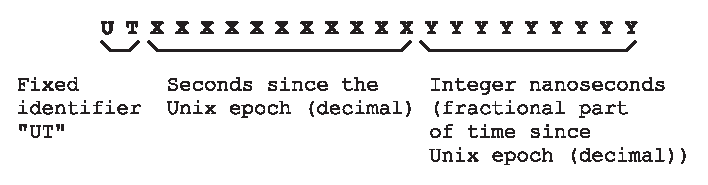
\includegraphics[width=4.6in]{utimeformat01.eps}
\caption{Format of UTIME}
\label{fig:stdd0:sdty0:sutm0:00}
\end{figure}

Figure \ref{fig:stdd0:sdty0:sutm0:00} illustrates the format of
an UTIME.  A UTIME consists of 22 characters, with the following
components.

\begin{itemize}
\item \textbf{``UT'' (2 characters):}
      This fixed string aids in preventing type accidents with
      string data types.
\item \textbf{Integer seconds since the Unix epoch (11 characters):}
      These 11 characters are an integer, zero-padded on the left as
      necessary, that represent the integer seconds since the Unix
      epoch.
\item \textbf{Nanoseconds associated with the integer seconds (9 characters):}
      These 9 characters are an integer, zero-padded on the left as
      necessary, that represent the nanoseconds associated with the
      integer seconds since the Unix
      epoch.  
\end{itemize}

Note that UTIMEs as described have the property that the lexical
string sort order corresponds to the time sort order.

Note that the UTIME format can be used only for values that:

\begin{itemize}
\item Are used as part of generating a unique or random data value
      (see, for example, \S{}\ref{stdd0:sdty0:sgui0}).
\item Are used to determine elapsed time.
\end{itemize}

UTIMEs cannot be mixed directly with scheduling time, as the FBO 
may be in a different time zone than the server.

%%%%%%%%%%%%%%%%%%%%%%%%%%%%%%%%%%%%%%%%%%%%%%%%%%%%%%%%%%%%%%%%%%%%%%%%%%%%%%%

\subsubsection{SGUID (Server Globally-Unique Identifier)}
\label{stdd0:sdty0:sgui0}

\index{SGUID}%
\index{globally-unique identifier}%
It is necessary or helpful in some contexts to have a way to create an
identifier that is guaranteed to occur no more often than once in the lifetime
of the server.  \emph{MySQL} can be used to create such identifiers, and there
are also methods based on file and IPC semantics that can be used.

The method used in the software is a \index{spin lock}spin lock on a precision
timestamp; and the timestamp is concatenated with the PID.  The method works
because:

\begin{itemize}
\item A single process (by virtue of the spin lock) can't generate the same
      precision timestamp twice.
\item No two processes can have the same PID at the same time.
\end{itemize}

\begin{figure}
\centering
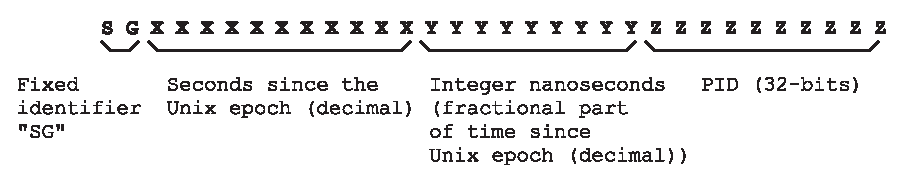
\includegraphics[width=4.6in]{sguidformat01.eps}
\caption{Format of SGUID}
\label{fig:stdd0:sdty0:sgui0:00}
\end{figure}

Figure \ref{fig:stdd0:sdty0:sgui0:00} illustrates the format of
an SGUID.  An SGUID consists of 32 characters, with the following
components.

\begin{itemize}
\item \textbf{``SG'' (2 characters):}
      This fixed string aids in preventing type accidents with
      string data types.
\item \textbf{Integer seconds since the Unix epoch (11 characters):}
      These 11 characters are an integer, zero-padded on the left as
      necessary, that represent the integer seconds since the Unix
      epoch.\footnote{Note that 11 digits comfortably solves the Unix
      2037 A.D. issue, as this will guarantee SGUIDs 
      beyond 5000 A.D.}
\item \textbf{Nanoseconds associated with the integer seconds (9 characters):}
      These 9 characters are an integer, zero-padded on the left as
      necessary, that represent the nanoseconds associated with the
      integer seconds since the Unix
      epoch.\footnote{As of this writing, Linux provides time to a resolution
      of microseconds.  It is anticipated that a resolution of nanoseconds will
      accommodate any hardware speed advances in the foreseeable future.}  
\item \textbf{PID (10 characters):}
      These 10 characters are an integer, zero-padded on the left as
      necessary, that represent Unix PID expressed 
      as a decimal number.\footnote{As of this writing, PIDs are 16 bits only.
      However, it seems inevitable that PIDs will be expanded to 24 or 32 bits in the 
      future.}  
\end{itemize}

Note that SGUIDs as described have a very important property---the lexical
string sort order corresponds to the time sort order, with the PID used as a tie-breaker.
This property is used to decide the priority of standby reservations 
(\S{}\ref{stdd0:ssby0}, p. \pageref{stdd0:ssby0}).

%%%%%%%%%%%%%%%%%%%%%%%%%%%%%%%%%%%%%%%%%%%%%%%%%%%%%%%%%%%%%%%%%%%%%%%%%%%%%%%

\subsubsection{SID (Session Identifier)}
\label{stdd0:sdty0:ssid0}

A \index{session identifier}session identifier (\index{SID}SID) is the
cookie provided to the browser to authenticate the user after a successful login
process is completed.

A session identifier is an identifier only.  The state associated with the
session is maintained on the server side.

A session identifier is exactly 66 characters long and consists of these components:

\begin{itemize}
\item The two characters ``SI'' (2 characters).
\item An SGUID as described in \S{}\ref{stdd0:sdty0:sgui0} (32 characters).
\item The server cryptographic hash function of the first two fields described
      above (32 characters).
\end{itemize}

The process of using an SID for authentication is protected by these mechanisms:

\begin{itemize}
\item It is impossible for a client to forge an SID, as the client does not have
      access to the server hash key.  (Additionally, it would be extremely for
      a client to guess an SGUID that is already associated with a session on the
      server, as this space is quite large.)
\item The \emph{\productbasename{}} software also records the IP address of the 
      connecting computer, records that information in the server-side session
      state, and will not accept the SID from a computer connecting from a different
      IP address.  Thus (NAT schemes aside) an SID cannot be reused by a client
      other than the one it was issued to.
\end{itemize}


%%%%%%%%%%%%%%%%%%%%%%%%%%%%%%%%%%%%%%%%%%%%%%%%%%%%%%%%%%%%%%%%%%%%%%%%%%%%%%%

\subsubsection{STIME (Scheduling Timestamp)}
\label{stdd0:sdty0:stim0}

\index{STIME}%
A scheduling timestamp is a timestamp in an abstract
calendar format with a resolution appropriate for:

\begin{itemize}
\item Representing the start times and end times of
      reservations.
\item Marking database records with a modification time that will be
      formatted and displayed.
\item Representing dates, such as expiration dates.
\end{itemize}

\begin{figure}
\centering
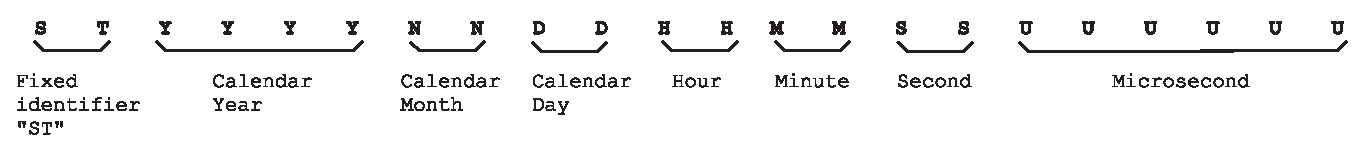
\includegraphics[width=4.6in]{stimeformat01.eps}
\caption{Format of STIME}
\label{fig:stdd0:sdty0:stim0:00}
\end{figure}

Figure \ref{fig:stdd0:sdty0:stim0:00} illustrates the format of
an STIME\@.  An STIME consists of 16 characters, with the following
components.

\begin{itemize}
\item \textbf{``ST'' (2 characters):}
      This fixed string aids in preventing type accidents with
      string data types.
\item \textbf{Calendar year (4 characters).}
\item \textbf{Calendar month (2 characters).}
\item \textbf{Calendar day (2 characters).}
\item \textbf{Hour, 24-hour time (2 characters).}
\item \textbf{Minute (2 characters).}
\item \textbf{Second (2 characters).}
\item \textbf{Microsecond (6 characters).}
\end{itemize}

Note that STIMEs as described have the property that the lexical
string sort order corresponds to the time sort order.

An STIME is used only for scheduling time, and is necessarily the time in the
client locale.


%%%%%%%%%%%%%%%%%%%%%%%%%%%%%%%%%%%%%%%%%%%%%%%%%%%%%%%%%%%%%%%%%%%%%%%%%%%%%%%

\subsubsection{DT8 (Short Calendar Date)}
\label{stdd0:sdty0:sdat8}

\index{DT8}%
The DT8 data type is used to specify dates in a shorthand
format in GET/POST parameters and in software internals.
The format is a string consisting of exactly 8
characters:

\begin{itemize}
\item Calendar year (4 characters).
\item Calendar month (2 characters).
\item Calendar day (2 characters).
\end{itemize}

A DT8 is used only for scheduling time, and is necessarily the time in the
client locale.


%%%%%%%%%%%%%%%%%%%%%%%%%%%%%%%%%%%%%%%%%%%%%%%%%%%%%%%%%%%%%%%%%%%%%%%%%%%%%%%

\subsubsection{T4 (Short Calendar Time)}
\label{stdd0:sdty0:sdtt4}

\index{T4}%
The T4 data type is used to specify times in a shorthand
format in GET/POST parameters and in software internals.
The format is a string consisting of exactly 4
characters:

\begin{itemize}
\item Hour (``00''-``23'', 2 characters).
\item Minute (``00''-``59'', 2 characters).
\end{itemize}

Note that the string ``2400'' is not a legal T4\@.  Technically, ``2400'' is
``0000'' of the following day.

A T4 is used only for scheduling time, and is necessarily the time in the
client locale.

%%%%%%%%%%%%%%%%%%%%%%%%%%%%%%%%%%%%%%%%%%%%%%%%%%%%%%%%%%%%%%%%%%%%%%%%%%%%%%%

\subsubsection{T3 (Shorter Calendar Time)}
\label{stdd0:sdty0:sdtt3}

\index{T3}%
The T3 data type is used to specify times in a shorthand
format in GET/POST parameters and in software internals, with
a granularity of 10 minutes.

Because \emph{\productbasename{}} will only schedule with a granularity
of 30 minutes, any start time of a reservation is expressible as a T3.

The format of a T3 is a string consisting of exactly 3
characters:

\begin{itemize}
\item Hour (``00''-``23'', 2 characters).
\item Minutes divided by ten (``0''-``5'', 1 character).
\end{itemize}

Note that the string ``240'' is not a legal T3\@.  Technically, ``240'' is
``000'' of the following day.

A T3 is used only for scheduling time, and is necessarily the time in the
client locale.

%%%%%%%%%%%%%%%%%%%%%%%%%%%%%%%%%%%%%%%%%%%%%%%%%%%%%%%%%%%%%%%%%%%%%%%%%%%%%%%

\subsubsection{T2 (Shortest Calendar Time)}
\label{stdd0:sdty0:sdtt2}

\index{T2}%
The T2 data type is used to specify times in a shorthand
format in GET/POST parameters and in software internals, with
a granularity of 1 hour.

A T2 is simply the hour of the time, and may range from ``00''-``23''.

Note that the string ``24'' is not a legal T2\@.  Technically, ``24'' is
``00'' of the following day.

A T2 is used only for scheduling time, and is necessarily the time in the
client locale.

%%%%%%%%%%%%%%%%%%%%%%%%%%%%%%%%%%%%%%%%%%%%%%%%%%%%%%%%%%%%%%%%%%%%%%%%%%%%%%%

\subsection{User Permissions}
\label{stdd0:supm0}

TBD.

%%%%%%%%%%%%%%%%%%%%%%%%%%%%%%%%%%%%%%%%%%%%%%%%%%%%%%%%%%%%%%%%%%%%%%%%%%%%%%%

\subsubsection{Permission Templates and Permission Schema}
\label{stdd0:supm0:snap0}

There are [at least] two ways of thinking about user permissions:

\begin{itemize}
\item A user is in a defined role (customer, FBO owner, line employee,
      flight instructor, etc.) and should have fixed privileges
      directly tied to to the role.
\item The role of the user is only a starting point for the granting
      of permissions.  Users may require more or fewer permissions, in
      a fine-grained sense, than is traditional for their role.  For example,
      a line employee may be authorized to change fuel prices or have other
      privileges not granted to other line employees.
\end{itemize}

The approach taken in the \emph{\productbasename{}} software is the second
approach---fine-grained permissions.  The specific approach taken is:

\begin{itemize}
\item At the time a user is created, they are created as a ``permission template'' corresponding
      to their role or job.  The permission template is a starting point.
\item Permissions are very specific and fine-grained, and all permissions can be
      individually added or removed from an individual user after the user
      account is created.
\item The permission templates and the associated permissions are 
      customizable in the configuration file.
\item Most user permissions are Boolean in nature, but some may have integer,
      floating point, or
      string values.
\end{itemize}


%%%%%%%%%%%%%%%%%%%%%%%%%%%%%%%%%%%%%%%%%%%%%%%%%%%%%%%%%%%%%%%%%%%%%%%%%%%%%%%

\subsubsection{Mechanism of Storage and Query}
\label{stdd0:supm0:sstq0}

PHP is an interpreted language.  The steps that are interpreted run
relatively slowly (because the interpreter must parse the PHP statements), whereas
PHP built-in functions (compiled `C' code) run very quickly.  One way to enhance
efficiency is to be sure that things that happen often come down to
built-in functions rather than PHP statements that must be interpreted.

SQL queries are also relatively slow, and a mechanism that avoids these
is desirable.

The mechanism chosen to represent permissions is:

\begin{itemize}
\item User permissions are represented as a single string (in \emph{MySQL}, a 
      \emph{varchar} field).
\item The user permission string is a group of permissions separated by
      the forward slash character (``/'').
\item Each permission takes one of the following forms:
      \begin{itemize}
      \item \emph{``/ptag''}: 
            For a boolean permission, presence of the
            \emph{ptag} indicates that the user has the permission, and absence
            of the \emph{ptag} indicates that the user does not have the permission.
      \item \emph{``/ptag=``value''}:
            The permission (or attribute) \emph{ptag} is assigned the
            \emph{value}.
      \end{itemize}
\item Permission strings are escaped so that the string \emph{``/ptag''}
      can occur only at the start of the definition of the permission
      \emph{ptag}.  Specifically:
      \begin{itemize}
      \item If the forward slash character occurs in the value of a
            permission, the forward slash character is escaped
            by suffixing it with the backslash character.
      \item The permission values allowed are very restrictive.  Specifically:
            \begin{itemize}
            \item Backslashes are not allowed within permission values.
            \item Double-quotes are not allowed within permission values.
            \end{itemize}
      \end{itemize}
\item Presence of a permission can be rapidly determined by using 
      a string search\footnote{The string search functions are built into PHP, and are
      very quick because they are compiled `C' code.}
      by ``\emph{/ptag}''.  Because of the escaping used,
      this string can only occur if permission \emph{ptag} exists.
\end{itemize}


%%%%%%%%%%%%%%%%%%%%%%%%%%%%%%%%%%%%%%%%%%%%%%%%%%%%%%%%%%%%%%%%%%%%%%%%%%%%%%%

\subsubsection{Administrator Permissions}
\label{stdd0:supm0:sadp0}

TBD.

%%%%%%%%%%%%%%%%%%%%%%%%%%%%%%%%%%%%%%%%%%%%%%%%%%%%%%%%%%%%%%%%%%%%%%%%%%%%%%%

\subsection{\emph{MySQL} Database Design}
\label{stdd0:smdd0}

TBD.

%%%%%%%%%%%%%%%%%%%%%%%%%%%%%%%%%%%%%%%%%%%%%%%%%%%%%%%%%%%%%%%%%%%%%%%%%%%%%%%

\subsubsection{Overall Relational Design}
\label{stdd0:srds0}

Figure \ref{fig:stdd0:srds0:00} illustrates the overall relational
database design.  The design consists conceptually of only five tables.
However, because the $\infty\leftrightarrow\infty$ relationships require
a cross-reference table, seven physical tables are actually required.

\begin{figure}
\centering
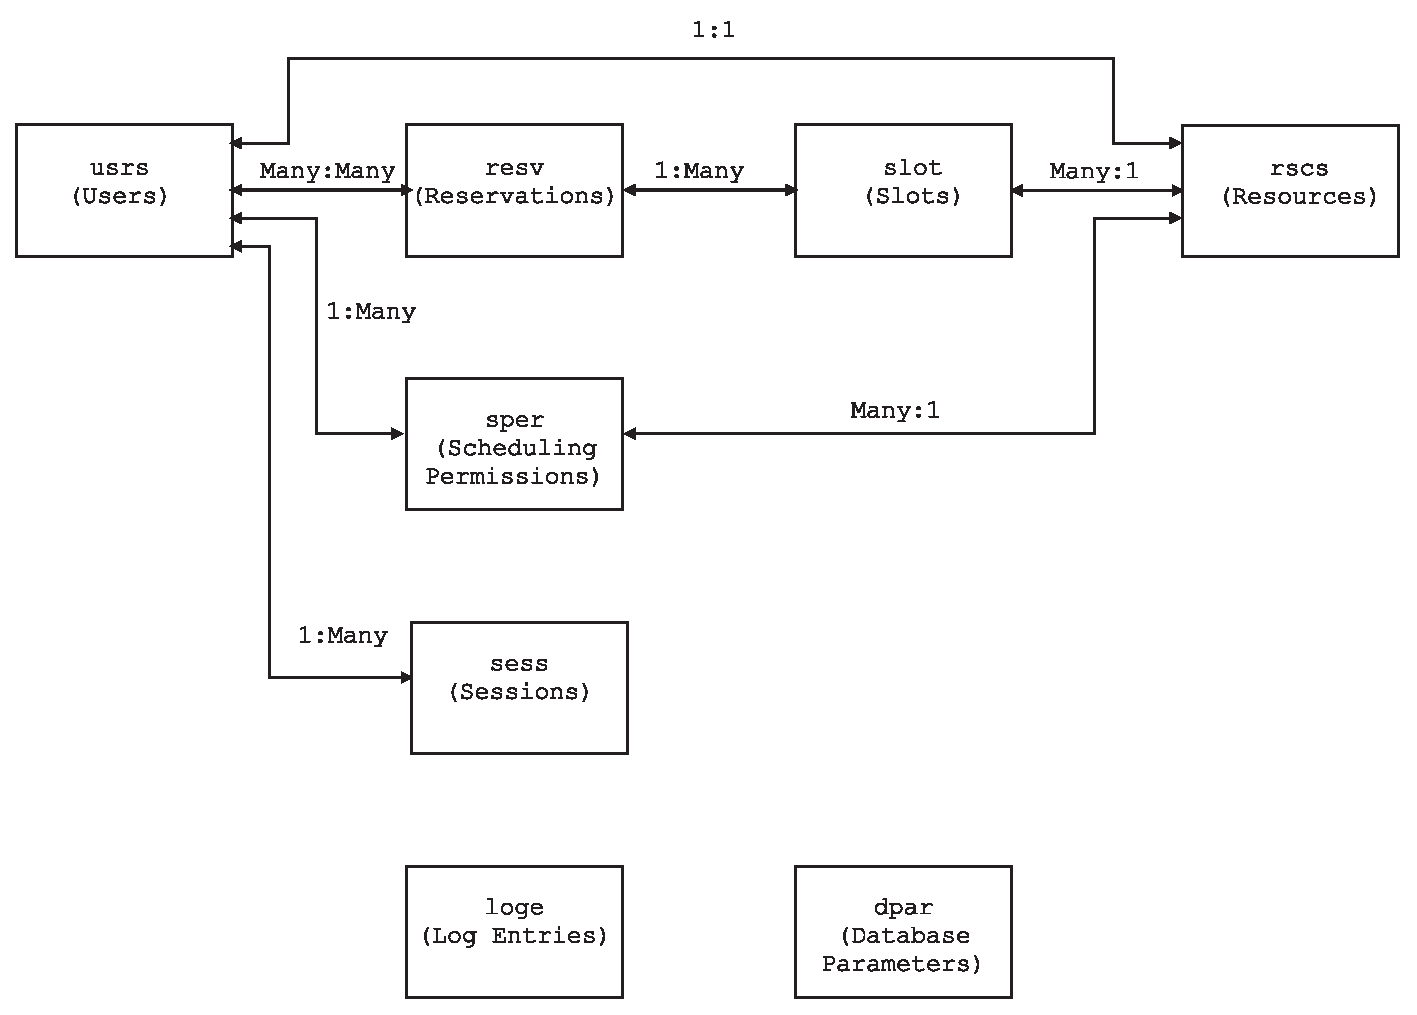
\includegraphics[width=4.6in]{rdoveralldesign01.eps}
\caption{\emph{\productname{}} Relational Database Overall Design}
\label{fig:stdd0:srds0:00}
\end{figure}

In the actual \emph{MySQL} database, the eight tables shown in 
Figure \ref{fig:stdd0:srds0:00} are named exactly
as indicated:  
\index{usrs@\emph{usrs}}\emph{usrs},  
\index{resv@\emph{resv}}\emph{resv}, 
\index{slot@\emph{slot}}\emph{slot},
\index{rscs@\emph{rscs}}\emph{rscs}, 
\index{sper@\emph{sper}}\emph{sper}, 
\index{sess@\emph{sess}}\emph{sess}, 
\index{loge@\emph{loge}}\emph{loge}, 
and 
\index{dpar@\emph{dpar}}\emph{dpar}.
The cross-reference table not shown in the figure is named by concatenating the 
cross-referenced table names:  
\index{usrsresv@\emph{usrsresv}}\emph{usrsresv}.

The seven tables shown in Figure \ref{fig:stdd0:srds0:00}
have the following contents:

\begin{itemize}
\item \textbf{\emph{usrs} (Users):}
      User information, including contact information and hashed password.
\item \textbf{\emph{resv} (Reservations):}
      Reservations, including comments.
\item \textbf{\emph{slot} (Slots):}
      Information about the actual time slot occupied by a reservations's
      linked resource, including start time and end time.\footnote{The
      \emph{slot} table allows a single reservation to use two or more different
      resources at different times.  This occurs most commonly when a student
      schedules both ``ground'' and ``air'' time with an instructor, and the
      ``ground'' time extends either before or after the ``air'' time, or both.}
\item \textbf{\emph{rscs} (Resources):}
      Schedulable resources, including aircraft, simulators, and flight instructors.
\item \textbf{\emph{sper} (Scheduling Permissions):}
      The relationship between users and resources, in terms of the user's ability
      to schedule the resource with and without an instructor.\footnote{Instructors themselves
      have no scheduling restrictions---any student may schedule time with any instructor.}
\item \textbf{\emph{sess} (Sessions):}
      State of user logins.
\item \textbf{\emph{loge} (Log entries):}
      Significant and insignificant events for the software.  These are stored
      in a database table rather than a file
      for easier sorting, viewing, manipulation, and pruning.
\item \textbf{\emph{dpar} (Database parameters):}
      Parameters of the database as a whole, such as the current
      version of \emph{\productbasename{}} that created the
      database and an SGUID obtained at the time any table of
      the database was modified.
\end{itemize}

Note in Figure \ref{fig:stdd0:srds0:00} that there is a 1:1 link indicated
between resources and users.  Every flight instructor resource is also a user, and so
when a user (usually, a student) creates, modifies, or cancels a reservation,
the flight instructor user may be automatically notified by e-mail.  In order to
determine the e-mail addresses associated with the flight instructor resource,
the link from the resource to the user is followed.  Without such a link, the
flight instructor's e-mail addresses would have to be maintained in two places in
the database.


%%%%%%%%%%%%%%%%%%%%%%%%%%%%%%%%%%%%%%%%%%%%%%%%%%%%%%%%%%%%%%%%%%%%%%%%%%%%%%%

\subsubsection{Structure of Reservations}
\label{stdd0:sres0}

A reservation consists of the following components (please
refer to Figure \ref{fig:stdd0:srds0:00}):

\begin{itemize}
\item One or more entries from the users table (\emph{usrs}).  In the case
      of multiple users attached to a reservation, all have authority to
      modify the reservation.
\item \textbf{Exactly one} record from the reservations table (\emph{resv}).
\item One or more entries from the slots table (\emph{slot}).
\item One or more entries from the resources table (\emph{rscs}), paired 
      1:1 with the entries from the slots table.  (Note also that a given reservation
      may include a given resource only once.)
\end{itemize}

The format of a \emph{reservation} as presented above is deliberately general.
It allows these reservation structures:

\begin{itemize}
\item More than one user may be included on a reservation.  This facilitates
      the case where two users schedule the same resource at the same time (for example,
      if two users fly together somewhere recreationally).
\item If more than one resource is included on a reservation, the resources need not be
      scheduled at the same time.  (For example, this accommodates the case where a student may have
      some ``ground'' time with a flight instructor before or after flying.)
\item Any number of resources may be present on a reservation.
      (For example, a mechanic could reserve three planes at once for reservations.)
\end{itemize}

Note that other rules (not related to database structure) may prohibit 
some of the structures above.  For example, a student may be prohibited
from scheduling more than one airplane and one instructor.

Zero-length reservations (reservations with $t_0 = t_1$) are currently prohibited.

Reservations can be of three types:

\begin{itemize}
\item \index{active reservation}\index{reservation!active}\textbf{Active Reservations:}
      An active reservation is a reservation that currently blocks a resource
      (prevents other simultaneous active reservations).
\item \index{standby reservation}\index{reservation!standby}\textbf{Standby Reservations:}
      A standby reservation is a reservation that can be promoted to
      an active reservation if the conflicting active reservation(s)
      are canceled.
\item \index{banner reservation}\index{reservation!banner}\textbf{Banner Reservations:}
      A banner reservation is a ``reservation'' that is for
      information only, and cannot block active reservations or be
      promoted to an active reservation.

      A banner reservation is for user information only.  Sample
      uses of banner reservations:

      \begin{itemize}
      \item To provide special instructions for scheduling an airplane
            or flight instructor.  (Example: ``\emph{Please contact Jane
            directly to schedule instruction on Mondays}''.)
      \item To provide information about an airplane or flight
            instructor.  (Example:  ``\emph{Rates have been
            increased to \$100/hr for this aircraft}''.)
      \end{itemize}
\end{itemize}

%%%%%%%%%%%%%%%%%%%%%%%%%%%%%%%%%%%%%%%%%%%%%%%%%%%%%%%%%%%%%%%%%%%%%%%%%%%%%%%

\subsubsection{Treatment of Standby Reservations}
\label{stdd0:ssby0}

A \index{standby reservation}\index{reservation!standby}\emph{standby reservation}
is a reservation made for resource(s) when the resource is/are already 
committed to another reservation(s) at the same time.  (\emph{At the same time} means
any form of overlap.)

A standby reservation is represented in exactly the same way as an
\index{active reservation}\index{reservation!active}active reservation, except that
the Boolean table field
\emph{isactive} (see \S{}\ref{sdtf0})
is set FALSE. 

Active and standby reservations are manipulated using the following
rules.

\begin{enumerate}
\item The maximum number (i.e. depth) of standby reservations is limited by
      a configuration constant in the \emph{TBD} file.  If this configuration
      constant is 0, standby reservations are not allowed.
\item The maximum depth of standby reservations configuration constant is 
      only loosely enforced.  There are some situations where depth of standby
      reservations will be underestimated (due to the computational complexity
      of evaluating the true depth), but \emph{at least} the number of configured
      standby reservations will be allowed.
\item When a user schedules a reservation, the reservation is created as an
      active reservation if there are no resource conflicts.  However, if there
      are resource conflicts and if the configuration allows it, the user is given the option of
      creating a standby reservation.
\item When an active reservation is canceled, one or more standby reservations will be
      automatically promoted, if applicable, to occupy the resources freed up.  If
      permission flags for the canceling user are appropriate, the promotion of standby
      reservations may be suppressed.
\item If a cancelation is made too close to the reservation time, (the notion of
      ``too close'' is a configuration constant), a standby reservation cannot be
      promoted (rationale:  not enough time for the person whose reservation is promoted
      to react).
\item FBO staff may change active reservations to standby reservations and may promote a 
      given standby reservation to active (thus changing all conflicting active
      reservations to standby reservations), 
      \textbf{but standby reservations may not have their priority reordered}.  
      The relative priority of multiple standby reservations is determined by the
      creation SGUID---this is an automatic assignment and cannot be changed manually.
\end{enumerate}


E-mail notifications are sent whenever:

\begin{itemize}
\item Standby reservations are automatically or manually
      promoted to active reservations.
\item A standby reservation can't be promoted to an active reservation
      because an active reservation was modified or deleted too close
      to the reservation time.
\end{itemize}

%%%%%%%%%%%%%%%%%%%%%%%%%%%%%%%%%%%%%%%%%%%%%%%%%%%%%%%%%%%%%%%%%%%%%%%%%%%%%%%

\subsection{Query Complexity}
\label{stdd0:sqcx0}

It needs to be verified that all of the intended queries and maintenance
operations are approximately $O(\log N)$ (see \S{}\ref{stbg0:sonn0}, p.
\pageref{stbg0:sonn0}).  In this section, the major queries are
examined in detail.


%%%%%%%%%%%%%%%%%%%%%%%%%%%%%%%%%%%%%%%%%%%%%%%%%%%%%%%%%%%%%%%%%%%%%%%%%%%%%%%

\subsubsection{Resource Scheduling Views}
\label{stdd0:sqcx0:ssvw0}

Scheduling views are perhaps the most important query.  Users expect
``snappy'' response (near-instant display of scheduling information).

A scheduling view is parameterized by:

\begin{itemize}
\item The set of resources whose schedules are to be displayed.
\item The time window, identified by a lower and an upper bound.
\end{itemize}

The set of resources whose scheduling information is to be displayed is a
linear constant.  It tends to be either of size one or every resource schedulable.
In any case, it is a small number ($<$100).

The time window is parameterized for an SQL query on key fields.

$O(\log N)$.

%%%%%%%%%%%%%%%%%%%%%%%%%%%%%%%%%%%%%%%%%%%%%%%%%%%%%%%%%%%%%%%%%%%%%%%%%%%%%%%

\subsubsection{User Views}
\label{stdd0:sqcx0:suvw0}

All conceivable user views and edits (alphabetical, uid, whatever) are
$O(\log N)$.  There may be a few deceptive queries that become $O(N)$, but these
can be massaged.

%%%%%%%%%%%%%%%%%%%%%%%%%%%%%%%%%%%%%%%%%%%%%%%%%%%%%%%%%%%%%%%%%%%%%%%%%%%%%%%

\subsubsection{Standby Reservations}
\label{stdd0:sqcx0:ssby0}




%%%%%%%%%%%%%%%%%%%%%%%%%%%%%%%%%%%%%%%%%%%%%%%%%%%%%%%%%%%%%%%%%%%%%%%%%%%%%%%

\subsection{Session Management}
\label{stdd0:ssmg0}

TBD.

%%%%%%%%%%%%%%%%%%%%%%%%%%%%%%%%%%%%%%%%%%%%%%%%%%%%%%%%%%%%%%%%%%%%%%%%%%%%%%%

\subsection{Mutual Exclusion and Database and Table Locking}
\label{stdd0:sdbl0}

\index{locking (database}\index{database locking}\emph{MySQL} guarantees that
each SQL statement will execute atomically.  In many cases, necessary actions
can be phrased as a single SQL statement, and no locking is required.  However, in
other cases, complex database updates must be completed atomically and locking
is required.

In addition to database design issues, editing collisions due to the nature
of HTTP must be handled appropriately.\footnote{Among web developers, these collisions
are sometimes called \emph{midair collisions}\@.  I don't believe
this is suitable nomenclature in an aviation environment, and so the
term \emph{HTTP editing collision} is used.}
An HTTP editing collision occurs when two [or more] users obtain copies of data
in web browser forms, one user commits changed data back, and the second user
commits different changes, with no knowledge of the changes made by the first user,
and thus may overwrite the first user's changes.

The strategy for mutual exclusion and database/table locking should meet
these requirements and constraints:

\begin{itemize}
\item The strategy must allow a database maintenance script to run concurrently
      with web access to the database.
\item The strategy must not block web page views for too long (never longer than 1-4 seconds,
      and no delay for the vast majority of web page accesses).
\item The strategy must be fair:  no process should block indefinitely.
\item The strategy should be simple.
\item The strategy must at least detect and optionally correct HTTP editing collisions. 
\end{itemize}

The strategy employed is:

\begin{itemize}
\item Any process (either maintenance or web access) that has mutual exclusion needs
      locks the entire database (rather than locking individual tables).
      \begin{itemize}
      \item This strategy is very simple.
      \item This strategy prevents the possibility of deadlock (due to ordering of table locks).
      \item This strategy inherently serializes and is fair (because of \emph{MySQL}'s behavior).
      \item Maintenance scripts can be written to check and correct the database
            incrementally and to lock the database only for short periods of time,
            thus not blocking web users for too long.
      \end{itemize}
\item In any scenario where an HTTP editing collision is a potential problem:
      \begin{itemize}
      \item An SGUID is stored on a database record commit.
      \item The SGUID is provided as a hidden form field on editing pages.
      \item At the time a commit is attempted, if the SGUID held by the browser is different than the
            one in the database, there has been an editing collision.  In this case, at minimum
            notification is made.
      \end{itemize}
\end{itemize}

Finally, database locking has the standard software problem of how to embed a critical
section within another critical section.  The pseudo-code below should suffice.

\begin{verbatim}
local_lock_var = global_lock_var;
lock_database();
global_lock_var = TRUE;

...
Take action, perhaps calling sub-functions with
identical pseudo-code.
...

if (! local_lock_var)
   {
   unlock_database();
   global_lock_var = FALSE;
   }
\end{verbatim}

%%%%%%%%%%%%%%%%%%%%%%%%%%%%%%%%%%%%%%%%%%%%%%%%%%%%%%%%%%%%%%%%%%%%%%%%%%%%%%%

\section{Web Pages}
\label{swpg0}

TBD.

%%%%%%%%%%%%%%%%%%%%%%%%%%%%%%%%%%%%%%%%%%%%%%%%%%%%%%%%%%%%%%%%%%%%%%%%%%%%%%%

\subsection{\texttt{index.php} (Scheduler Entry Page / All Scheduling Views)}
\label{swpg0:siph0}

TBD.

%%%%%%%%%%%%%%%%%%%%%%%%%%%%%%%%%%%%%%%%%%%%%%%%%%%%%%%%%%%%%%%%%%%%%%%%%%%%%%%

\subsection{\texttt{logview.php} (Action / Event / Exception Log View)}
\label{swpg0:slvw0}

TBD.

%%%%%%%%%%%%%%%%%%%%%%%%%%%%%%%%%%%%%%%%%%%%%%%%%%%%%%%%%%%%%%%%%%%%%%%%%%%%%%%

\subsection{\texttt{resourceadd.php} (Resource Addition)}
\label{swpg0:srad0}

TBD.

%%%%%%%%%%%%%%%%%%%%%%%%%%%%%%%%%%%%%%%%%%%%%%%%%%%%%%%%%%%%%%%%%%%%%%%%%%%%%%%

\subsection{\texttt{resourceedit.php} (Resource Edit)}
\label{swpg0:sred0}

TBD.

%%%%%%%%%%%%%%%%%%%%%%%%%%%%%%%%%%%%%%%%%%%%%%%%%%%%%%%%%%%%%%%%%%%%%%%%%%%%%%%

\subsection{\texttt{resourcemanage.php} (Resource List / Select Action)}
\label{swpg0:srmg0}

TBD.

%%%%%%%%%%%%%%%%%%%%%%%%%%%%%%%%%%%%%%%%%%%%%%%%%%%%%%%%%%%%%%%%%%%%%%%%%%%%%%%

\subsection{\texttt{resourceview.php} (Resource View)}
\label{swpg0:srvw0}

TBD.

%%%%%%%%%%%%%%%%%%%%%%%%%%%%%%%%%%%%%%%%%%%%%%%%%%%%%%%%%%%%%%%%%%%%%%%%%%%%%%%

\subsection{\texttt{signupadd.php} (Signup Addition)}
\label{swpg0:ssad0}

TBD.

%%%%%%%%%%%%%%%%%%%%%%%%%%%%%%%%%%%%%%%%%%%%%%%%%%%%%%%%%%%%%%%%%%%%%%%%%%%%%%%

\subsection{\texttt{signupedit.php} (Signup Edit)}
\label{swpg0:ssed0}

TBD.

%%%%%%%%%%%%%%%%%%%%%%%%%%%%%%%%%%%%%%%%%%%%%%%%%%%%%%%%%%%%%%%%%%%%%%%%%%%%%%%

\subsection{\texttt{signupmanage.php} (Signup List / Select Action)}
\label{swpg0:ssmg0}

TBD.

%%%%%%%%%%%%%%%%%%%%%%%%%%%%%%%%%%%%%%%%%%%%%%%%%%%%%%%%%%%%%%%%%%%%%%%%%%%%%%%

\subsection{\texttt{signupview.php} (Signup View)}
\label{swpg0:ssvw0}

TBD.

%%%%%%%%%%%%%%%%%%%%%%%%%%%%%%%%%%%%%%%%%%%%%%%%%%%%%%%%%%%%%%%%%%%%%%%%%%%%%%%

\subsection{\texttt{useradd.php} (User Addition)}
\label{swpg0:susd0}

TBD.

%%%%%%%%%%%%%%%%%%%%%%%%%%%%%%%%%%%%%%%%%%%%%%%%%%%%%%%%%%%%%%%%%%%%%%%%%%%%%%%

\subsection{\texttt{useredit.php} (User Edit)}
\label{swpg0:suse0}

TBD.

%%%%%%%%%%%%%%%%%%%%%%%%%%%%%%%%%%%%%%%%%%%%%%%%%%%%%%%%%%%%%%%%%%%%%%%%%%%%%%%

\subsection{\texttt{useremail.php} (Send Mass E-mail / Announcement to Users)}
\label{swpg0:seus0}

TBD.

%%%%%%%%%%%%%%%%%%%%%%%%%%%%%%%%%%%%%%%%%%%%%%%%%%%%%%%%%%%%%%%%%%%%%%%%%%%%%%%

\subsection{\texttt{usermanage.php} (User List / Select Action)}
\label{swpg0:sumg0}

TBD.

%%%%%%%%%%%%%%%%%%%%%%%%%%%%%%%%%%%%%%%%%%%%%%%%%%%%%%%%%%%%%%%%%%%%%%%%%%%%%%%

\subsection{\texttt{userview.php} (User View)}
\label{swpg0:suvw0}

TBD.

%%%%%%%%%%%%%%%%%%%%%%%%%%%%%%%%%%%%%%%%%%%%%%%%%%%%%%%%%%%%%%%%%%%%%%%%%%%%%%%

\section{Standalone Scripts}
\label{ssas0}

TBD.

%%%%%%%%%%%%%%%%%%%%%%%%%%%%%%%%%%%%%%%%%%%%%%%%%%%%%%%%%%%%%%%%%%%%%%%%%%%%%%%

\subsection{\texttt{adminforce.php} (Emergency Administrator Password Reset)}
\label{ssas0:samf0}

TBD.

%%%%%%%%%%%%%%%%%%%%%%%%%%%%%%%%%%%%%%%%%%%%%%%%%%%%%%%%%%%%%%%%%%%%%%%%%%%%%%%

\subsection{\texttt{dbconncheck.php} (Database Connectivity and Authentication Check)}
\label{ssas0:sdbc0}

\index{dbconncheck.php@\texttt{dbconncheck.php}}The \texttt{dbconncheck.php}
script takes the following actions:

\begin{itemize}
\item Attempts to connect and authenticate to the \emph{MySQL} daemon
      using the information in 
      \index{config.inc@\texttt{config.inc}}\texttt{config.inc}.
\item Attempts to select the database specified in the 
      \texttt{config.inc}.
\item Attempts to close the \emph{MySQL} connection.
\item Announces failure or success and provides details.
\end{itemize}

The \texttt{dbconncheck.php} can be used to verify \emph{MySQL} database connectivity
during the \emph{\productbasename{}} setup process.

The \texttt{dbconncheck.php} script takes no command-line parameters (it receives
the \emph{MySQL} connection it requires by including \emph{PHP} library files).


%%%%%%%%%%%%%%%%%%%%%%%%%%%%%%%%%%%%%%%%%%%%%%%%%%%%%%%%%%%%%%%%%%%%%%%%%%%%%%%

\subsection{\texttt{dbinit.php} (Database Initialization and Upgrade)}
\label{ssas0:sdbi0}

TBD.

%%%%%%%%%%%%%%%%%%%%%%%%%%%%%%%%%%%%%%%%%%%%%%%%%%%%%%%%%%%%%%%%%%%%%%%%%%%%%%%

\subsection{\texttt{mainthot.php} (In-Service Daily Database Maintenance)}
\label{ssas0:smah0}

TBD.

%%%%%%%%%%%%%%%%%%%%%%%%%%%%%%%%%%%%%%%%%%%%%%%%%%%%%%%%%%%%%%%%%%%%%%%%%%%%%%%

\subsection{\texttt{phplibset.php} (Source File PHP Library Path Modification)}
\label{ssas0:sphl0}

TBD.

%%%%%%%%%%%%%%%%%%%%%%%%%%%%%%%%%%%%%%%%%%%%%%%%%%%%%%%%%%%%%%%%%%%%%%%%%%%%%%%

\subsection{\texttt{sitehashkeygen.php} (Source Hash Key Generation)}
\label{ssas0:shkg0}

The \index{sitehashkeygen.php@\emph{sitehashkeygen.php}}\texttt{sitehashkeygen.php}
script generates a suitable site hash key as a constant in a PHP include file
and places it in a file named \emph{sitehashkey.inc}.

By default, the \emph{sitehashkey.inc} is placed in the current working directory.
However, the \texttt{sitehashkeygen.php} script accepts an optional parameter,
the directory in which to place the file.

\begin{figure}
\begin{scriptsize}
\begin{verbatim}
<?php
//This PHP include file contains the FboPrime site hash key.  This key is
//normally automatically generated at the time the software is set up.
//This key can be edited by hand safely--it is just an ordinary string of
//arbitrary length.  However, if it is manually edited, it should be
//edited only at the time the system is set up.  Modifying this key on a
//working system will invalidate every user password and may have other ill
//effects as well.
//
//Permissions on this file should be set so that FboPrime users cannot view
//its contents (it should be private to the Apache server).  If FboPrime
//users can view this key, it may enable some security attacks on the
//FboPrime software (as users may be able to forge some data).
//
//Generating program:                    $RCSfile: manual.tex,v $
//Generating program CVS revision:       $Revision: 1.36 $
//Generating program CVS revision date:  $Date: 2006/04/10 04:28:07 $
//Time of key generation:                05-Feb-2006 14:15:26 (UTC -0500)
//------------------------------------------------------------------------------------------
define("SITEHASHKEY_SITEHASHKEY", "5bc9fc5b2fafd50c5ac9c267f03fecb1668cf4de80f37f392b" .
                                  "2fbe0fefd0e5f76G[o6BCR.pitb[z-GOgdk=3GzdwU=I2)8>ff" .
                                  "vS(s17Wc,f?F*fS70WOz<3dUMfLV9=<FCZ[D(OQ/-PtQ*5Y*=w" .
                                  "nUzAy5Q3_Z*ToqCg*r*DgRbJq?O8*zEad.LL2kO-3CGr+1HPtv" );
?>
\end{verbatim}
\end{scriptsize}
\caption{Format of Automatically-Generated \emph{sitehashkey.inc} File}
\label{fig:ssas0:shkg0:00}
\end{figure}

A typical automatically-generated 
\emph{sitehashkey.inc} file is shown in Figure \ref{fig:ssas0:shkg0:00}.

%%%%%%%%%%%%%%%%%%%%%%%%%%%%%%%%%%%%%%%%%%%%%%%%%%%%%%%%%%%%%%%%%%%%%%%%%%%%%%%

\subsection{\texttt{sbyrespromote.php} (Promotion of Standby Reservations)}
\label{ssas0:spsr0}

TBD.

%%%%%%%%%%%%%%%%%%%%%%%%%%%%%%%%%%%%%%%%%%%%%%%%%%%%%%%%%%%%%%%%%%%%%%%%%%%%%%%

\section{PHP Library Files}
\label{sphl0}

TBD.

%%%%%%%%%%%%%%%%%%%%%%%%%%%%%%%%%%%%%%%%%%%%%%%%%%%%%%%%%%%%%%%%%%%%%%%%%%%%%%%

\subsection{\texttt{config.inc} (Global Configuration Constants)}
\label{sphl0:siph0}

\index{config.inc@\texttt{config.inc}}The \texttt{config.inc} file contains particulars
of the FBO and the installation, including:

\begin{itemize}
\item FBO location and contact information (mailing address, phone numbers, etc.).
\item Database connection information (host, database, userid, and password information).
\item Behavioral constants (scheduling and data retention policy).
\end{itemize}

This file must be customized as part of the
\emph{\productbasename{}} installation process.

%%%%%%%%%%%%%%%%%%%%%%%%%%%%%%%%%%%%%%%%%%%%%%%%%%%%%%%%%%%%%%%%%%%%%%%%%%%%%%%

\subsection{\texttt{confighard.inc} (Global Unmodifyable Configuration Constants)}
\label{sphl0:scfh1}

\index{confighard.inc@\texttt{confighard.inc}}The \texttt{confighard.inc} file contains
global configuration constants that either:

\begin{itemize}
\item Would not need to be configured by the FBO, or
\item Are bound tightly to the code and so can't be changed without also
      changing the code.
\end{itemize}

The constants in this file should not be changed by the users of the
\emph{\productbasename{}} software.

%%%%%%%%%%%%%%%%%%%%%%%%%%%%%%%%%%%%%%%%%%%%%%%%%%%%%%%%%%%%%%%%%%%%%%%%%%%%%%%

\subsection{\texttt{crhsh.inc} (Cryptographic Hash Functions)}
\label{sphl0:schf0}

\index{crhsh.inc@\texttt{crhsh.inc}}The \texttt{crhsh.inc} file 
contains functions dealing with cryptographic hashes.

See \S{}\ref{stbg0:smdf0}, \S{}\ref{stbg0:sfch0}, and \S{}\ref{stbg0:spst0}.

%%%%%%%%%%%%%%%%%%%%%%%%%%%%%%%%%%%%%%%%%%%%%%%%%%%%%%%%%%%%%%%%%%%%%%%%%%%%%%%

\subsection{\texttt{datefunc.inc} (Date Calculation and Related Functions)}
\label{sphl0:sdfc0}

\index{datefunc.inc@\texttt{datefunc.inc}}The \texttt{datefunc.inc} file 
contains functions that perform date calculations
(for example, date differences and the day of the week corresponding
to an arbitrary date).  Many of the calculations are based on modulo
arithmetic.

%%%%%%%%%%%%%%%%%%%%%%%%%%%%%%%%%%%%%%%%%%%%%%%%%%%%%%%%%%%%%%%%%%%%%%%%%%%%%%%

\subsection{\texttt{sitehashkey.inc} (Site Hash Key)}
\label{sphl0:sshk0}

\index{sitehaskey.inc@\texttt{sitehashkey.inc}}The \texttt{sitehashkey.inc} file contains
the site hash key.  This file is normally automatically generated by the
\index{sitehashkeygen.php@\emph{sitehashkeygen.php}}\texttt{sitehashkeygen.php}
script as part of the \emph{\productbasename{}} installation process.

Please see:

\begin{itemize}
\item \S{}\ref{sins0:sssi0:sgsh0} (p. \pageref{sins0:sssi0:sgsh0})
      for instructions about how to execute the \texttt{sitehashkeygen.php}
      script to generate the \texttt{sitehashkey.inc} file.
\item \S{}\ref{ssas0:shkg0} (p. \pageref{ssas0:shkg0})
      for a description of the \texttt{sitehashkeygen.php}
      script.
\item Fig. \ref{fig:ssas0:shkg0:00} (p. \pageref{fig:ssas0:shkg0:00})
      for the typical format of a site hash key.
\end{itemize}

%%%%%%%%%%%%%%%%%%%%%%%%%%%%%%%%%%%%%%%%%%%%%%%%%%%%%%%%%%%%%%%%%%%%%%%%%%%%%%%

\subsection{\texttt{timeraw.inc} (Raw Time Acquisition)}
\label{sphl0:strw0}

\index{timeraw.inc@\texttt{timeraw.inc}}The \texttt{timeraw.inc} file contains
functions that obtain the raw time from the server's clock.

Functions that obtain the raw time are localized in one file to ease
Unix epoch issue changes if they have to be made.

%%%%%%%%%%%%%%%%%%%%%%%%%%%%%%%%%%%%%%%%%%%%%%%%%%%%%%%%%%%%%%%%%%%%%%%%%%%%%%%

\subsection{\texttt{utime.inc} (UTIME Acquisition and Operations)}
\label{sphl0:sutm0}

\index{utime.inc@\texttt{utime.inc}}The \texttt{utime.inc} file contains
functions that:

\begin{itemize}
\item Obtain the raw time from the server's clock in the UTIME
      format (described in \S{}\ref{stdd0:sdty0:sutm0}).
\item Perform operations on the UTIME data type
      (described in \S{}\ref{stdd0:sdty0:sutm0}).
\end{itemize}

%%%%%%%%%%%%%%%%%%%%%%%%%%%%%%%%%%%%%%%%%%%%%%%%%%%%%%%%%%%%%%%%%%%%%%%%%%%%%%%

\clearpage{}
\section{\emph{MySQL} Database Tables and Fields}
\label{sdtf0}

This section provides a detailed description of each \emph{MySQL} database table
and field.  Documentation is maintained in this document rather than in
the software source code.

%%%%%%%%%%%%%%%%%%%%%%%%%%%%%%%%%%%%%%%%%%%%%%%%%%%%%%%%%%%%%%%%%%%%%%%%%%%%%%%
\subsection{\emph{usrs} (Users) Table}
\label{sdtf0:susr0}

The \emph{usrs} table contains information about each user, with each user stored in
one database row.

\begin{docdbtblfielddef}

\item \index{uidx@\emph{uidx}}\textbf{\emph{uidx} (int)}

An integer index identifying the user, automatically assigned by the
\emph{MySQL} database.

In many contexts (GET and POST parameters, for example), this index is
used to identify a user.  It provides a generally shorter way to identify
a user than the \emph{userid}.

\item \index{userid@\emph{userid}}\textbf{\emph{userid} (varchar[20])}

The text string used to log in to the 
\emph{\productbasename{}} software.  In the database table,
this string is always stored in lower-case, but the software treats
this string as case-insensitive when it is entered by a user.

This string must begin with a letter, and may contain letters and
digits only.

The FBO may assign this text string arbitrarily.  Common conventions
are to use the first initial and last name (example: \emph{dashley}), 
first and middle initial and last name (example: \emph{dtashley}),
or a nickname (example: \emph{womanizer}).
\end{docdbtblfielddef}


%%%%%%%%%%%%%%%%%%%%%%%%%%%%%%%%%%%%%%%%%%%%%%%%%%%%%%%%%%%%%%%%%%%%%%%%%%%%%%%
\subsection{\emph{resv} (Reservations) Table}
\label{sdtf0:srsv0}

\index{resv@\emph{resv}}The 
\emph{resv} table contains one record for each reservation.

\begin{docdbtblfielddef}
\item \index{ridx@\emph{ridx}}\textbf{\emph{ridx} (int64)}

An integer index identifying the reservation, automatically
assigned by the \emph{MySQL} database.

\item \index{sstime@\emph{sstime}}\textbf{\emph{sstime} (char[14])}

An STIME string identifying the start time of the reservation.  This is 
necessarily the minimum of the start times of any of the \emph{slot}s linked
to the reservation, and is used to facilitate more efficient queries.

\item \index{estime@\emph{estime}}\textbf{\emph{estime} (char[14])}

An STIME string identifying the end time of the reservation.  This is 
necessarily the maximum of the end times of any of the \emph{slot}s linked
to the reservation, and is used to facilitate more efficient queries.

\item \index{csguid@\emph{csguid}}\textbf{\emph{csguid} (SGUID)}

An SGUID assigned at the time the reservation is created.  This provides
information about when the reservation is created, and also provides a
guaranteed unique sort order for standby reservations.

\item \index{msguid@\emph{msguid}}\textbf{\emph{msguid} (SGUID)}

An SGUID assigned at the time the reservation is created or modified.
This is used to prevent editing collisions and double-commits.

\item \index{isactive@\emph{isactive}}\textbf{\emph{isactive} (BOOLEAN)}

TRUE if the reservation is an
\index{active reservation}\index{reservation!active}active reservation,
or FALSE if the reservation is a standby reservation. 
\end{docdbtblfielddef}

%%%%%%%%%%%%%%%%%%%%%%%%%%%%%%%%%%%%%%%%%%%%%%%%%%%%%%%%%%%%%%%%%%%%%%%%%%%%%%%
\subsection{\emph{slot} (Slots) Table}
\label{sdtf0:sslt0}

\index{slot@\emph{slot}}

TBD.

%%%%%%%%%%%%%%%%%%%%%%%%%%%%%%%%%%%%%%%%%%%%%%%%%%%%%%%%%%%%%%%%%%%%%%%%%%%%%%%
\subsection{\emph{rscs} (Resources) Table}
\label{sdtf0:srsc0}

\index{rscs@\emph{rscs}}

TBD.

%%%%%%%%%%%%%%%%%%%%%%%%%%%%%%%%%%%%%%%%%%%%%%%%%%%%%%%%%%%%%%%%%%%%%%%%%%%%%%%
\subsection{\emph{sper} (Scheduling Permissions) Table}
\label{sdtf0:sspr0}

\index{sper@\emph{sper}}

TBD.

%%%%%%%%%%%%%%%%%%%%%%%%%%%%%%%%%%%%%%%%%%%%%%%%%%%%%%%%%%%%%%%%%%%%%%%%%%%%%%%
\subsection{\emph{sess} (Sessions) Table}
\label{sdtf0:sses0}

\index{sess@\emph{sess}}

TBD.

%%%%%%%%%%%%%%%%%%%%%%%%%%%%%%%%%%%%%%%%%%%%%%%%%%%%%%%%%%%%%%%%%%%%%%%%%%%%%%%
\subsection{\emph{loge} (Log Entries) Table}
\label{sdtf0:slge0}

\index{loge@\emph{loge}}

TBD.

%%%%%%%%%%%%%%%%%%%%%%%%%%%%%%%%%%%%%%%%%%%%%%%%%%%%%%%%%%%%%%%%%%%%%%%%%%%%%%%
\subsection{\emph{dpar} (Database Parameters) Table}
\label{sdtf0:sdpr0}

\index{dpar@\emph{dpar}}

TBD.


%%%%%%%%%%%%%%%%%%%%%%%%%%%%%%%%%%%%%%%%%%%%%%%%%%%%%%%%%%%%%%%%%%%%%%%%%%%%%%%

\clearpage{}
\section{User Permission Flags and Values}
\label{supf0}

\begin{docdbtblfielddef}

\item \index{slvl@\emph{slvl}}\textbf{\emph{slvl} (Security Level)}

      The general security level of the user.  Security levels are in descending
      security order.  In general, a user at security level $n$ 
      cannot modify the settings of users with security level $<n$.

      The levels used are:

      \begin{itemize}
      \item \textbf{0:}
            System administrators.
      \item \textbf{1:}
            FBO management and senior staff.
      \item \textbf{2:}
            Flight instructors and mechanics.
      \item \textbf{3:}
            Line employees.
      \item \textbf{4:}
            Customers.
      \end{itemize}

\end{docdbtblfielddef}

%%%%%%%%%%%%%%%%%%%%%%%%%%%%%%%%%%%%%%%%%%%%%%%%%%%%%%%%%%%%%%%%%%%%%%%%%%%%%%%

\clearpage{}
\section{Glossary of Database Parameters}
\label{sgld0}

This glossary describes the parameters that may be stored in the 
\emph{dpar} database table (see \S{}\ref{sdtf0:sdpr0}).

\begin{docglossaryenum}
\item \index{MAINT_SCRIPT_ACTIVE@\emph{MAINT\_SCRIPT\_ACTIVE}}\textbf{MAINT\_SCRIPT\_ACTIVE}

      Has the value of `0' if the maintenance script is not active, or 
      the value of a UTIME (described in \S{}\ref{stdd0:sdty0:sutm0}) representing
      the time at which the maintenance script was started if the
      maintenance script is active.
      
      This parameter is used 
      so that a second instance of the maintenance script cannot be started while 
      an earlier invocation is still in progress.

      This parameter is also used to detect when a maintenance script has
      been terminated abormally, so that future invocations are not
      blocked indefinitely.  The criterion used is that the maintenance
      script has apparently been active for too long (this can easily
      be determined from the UTIME value).

\item \index{FBOPRIME_VERSION@\emph{FBOPRIME\_VERSION}}\textbf{FBOPRIME\_VERSION}

      The version number of \emph{\productbasename{}} that created the database.
      This version number is used only for database upgrades.
      The version of \emph{\productbasename{}} described by this document is 
      \emph{\productversion{}}.
\end{docglossaryenum}


%%%%%%%%%%%%%%%%%%%%%%%%%%%%%%%%%%%%%%%%%%%%%%%%%%%%%%%%%%%%%%%%%%%%%%%%%%%%%%%

\clearpage{}
\section{Glossary of GET/POST Parameters}
\label{sglo0}

TBD.

%%%%%%%%%%%%%%%%%%%%%%%%%%%%%%%%%%%%%%%%%%%%%%%%%%%%%%%%%%%%%%%%%%%%%%%%%%%%%%%

\clearpage{}
\section{Glossary of Terms, Acronyms, and Nomenclature}
\label{sglo1}

\begin{docglossaryenum}

\item \index{GMT}\textbf{GMT}

      See \emph{UTC} in this section.

\item \textbf{MAC}\index{MAS@\emph{MAC}}

      Marshall Aviation Center.

\item \textbf{MAS}\index{MAS@\emph{MAS}}

      Metzger's Aircraft Services.

\item \index{UTC}\textbf{UTC}

      \emph{UTC} (universal time)
      is the time kept on the Greenwich meridian (longitude zero), and is 
      normally five hours ahead of 
      \index{Eastern Standard Time}Eastern Standard Time (\index{EST}EST).
      UTC is sometimes also called 
      \index{GMT}GMT (\index{Greenwich Mean Time}Greenwich Mean Time)
      or \index{Zulu time}Zulu time.

\end{docglossaryenum}


%%%%%%%%%%%%%%%%%%%%%%%%%%%%%%%%%%%%%%%%%%%%%%%%%%%%%%%%%%%%%%%%%%%%%%%%%%%%%%%
\clearpage{}
\addcontentsline{toc}{section}{References}

\begin{thebibliography}{000}
\bibitem{bibref:com:kalsoft}
   \index{Kalamazoo Software}\emph{Kalamazoo Software}\\
   \texttt{http://www.kal-soft.com}
\bibitem{bibref:i:masternakdawn}
   \index{Masternak, Dawn}\emph{Dawn Masternak}\\
   \texttt{d\_masternak@hotmail.com}
\bibitem{bibref:i:whitingtheresa}
   \index{Whiting, Theresa}\emph{Theresa Whiting}\\
   \texttt{limeshoes@yahoo.com}
\bibitem{bibref:i:wynjadaniel}
   \index{Wynja, Daniel}\emph{Daniel Wynja}\\
   \texttt{danielwynja@hotmail.com}
\bibitem{bibref:i:metzgereric}
   \index{Metzger, Eric}\emph{Eric Metzger}\\
   \texttt{ericmetzger@charter.net}
\bibitem{bibref:i:ashleydavidt}
   \index{Ashley, David}\emph{Ashley, David}\\
   \texttt{dta@e3ft.com}
\bibitem{bibref:p:ors}
   \index{ORS@\emph{ORS}}\emph{ORS} (\emph{O}nline \emph{R}esource \emph{S}cheduler)\\
   \texttt{http://ors.sourceforge.net}
\bibitem{bibref:hagenhostingweb}
   \index{Hagen Hosting}\emph{Hagen Hosting}\\
   \texttt{http://www.hagenhosting.com}
\bibitem{bibref:c:mysql}
   \index{MySQL@\emph{MySQL}}\emph{MySQL} \\
   \texttt{http://www.mysql.com}
\bibitem{bibref:annarboraviationcenterweb}
   \emph{Ann Arbor Aviation Center} \\
   \texttt{http://www.aviationcenter.aero}
\bibitem{bibref:gnuorgweb}
   \emph{GNU} \\
   \texttt{http://www.gnu.org}
\bibitem{bibref:rfc1321}
   \index{RFC 1321}\index{MD5 message digest algorithm}\emph{RFC 1321---The MD5 Message-Digest Algorithm} \\
   \texttt{http://www.faqs.org/rfcs/rfc1321.html}
\bibitem{bibref:i:rostamianrouben}
   \index{Rostamian, Rouben}\emph{Rouben Rostamian}\\
   \texttt{rouben@pc18.math.umbc.edu}
\end{thebibliography}

%%%%%%%%%%%%%%%%%%%%%%%%%%%%%%%%%%%%%%%%%%%%%%%%%%%%%%%%%%%%%%%%%%%%%%%%%%%%%%%
\clearpage{}
\addcontentsline{toc}{section}{Index}
\printindex
%%%%%%%%%%%%%%%%%%%%%%%%%%%%%%%%%%%%%%%%%%%%%%%%%%%%%%%%%%%%%%%%%%%%%%%%%%%%%%%
\end{document}
%
%$Log: manual.tex,v $
%Revision 1.36  2006/04/10 04:28:07  dashley
%Edits.
%
%Revision 1.35  2006/04/08 04:03:02  dashley
%Edits.
%
%Revision 1.34  2006/04/08 00:25:11  dashley
%Edits.
%
%Revision 1.33  2006/04/05 02:04:35  dashley
%Edits.
%
%Revision 1.32  2006/04/02 23:18:42  dashley
%Edits.
%
%End of $RCSfile: manual.tex,v $.

